\chapter{Hybrid Memory Architectures}\label{ch:hybrid}

The previous chapters studied two kinds of sequence memory in isolation. Softmax attention
(\cref{ch:foundations}) keeps every past token as a key--value pair. Its recall is exact and
flexible, but the key--value (KV) cache grows linearly with the context and every decoding step
reads all of it. Linear attention, state space models (SSMs) and the delta-rule family
(\cref{ch:linear,ch:delta}) instead squeeze the whole past into a matrix of fixed size. They
decode in constant time and memory per token, but a fixed-size state cannot hold an unbounded
number of facts, so precise recall of an arbitrary old token eventually fails.

A \emph{hybrid} architecture puts both memories in one network. Some layers, or some heads
inside a layer, use attention for high-resolution recall; the others use a recurrent state for
cheap, compressed context. This is now the mainstream way to build efficient long-context
models: the survey's Section~V-A \citep{zhoubian2026memory} lists fixed serial hybrids (Kimi
Linear, OLMo Hybrid), hybrid-head models (Hymba, Falcon-H1), conversions of pre-trained
Transformers (LightTransfer, Priming), retrieval-augmented hybrids (Expansion Span) and
multi-component designs (Hydra). This chapter explains why the combination works, lays out the
design space, and then walks through eight 2025--2026 systems and their code.

\paragraph{Roadmap.} \Cref{sec:c12-background} builds the background: attention and recurrent
layers as two associative memories, a precise statement of the recall--efficiency trade-off,
and the design space (serial versus parallel mixing, hybrid ratio, placement, KV sharing,
training from scratch versus conversion). The system sections follow: Hybrid Quadratic-Linear
Transformers (\cref{sec:c12-hqlt}), Hymba (\cref{sec:c12-hymba}), Falcon-H1
(\cref{sec:c12-falcon}), the systematic study of hybrid linear attention
(\cref{sec:c12-analysis}), OLMo Hybrid (\cref{sec:c12-olmo}), Expansion Span
(\cref{sec:c12-expansion}), Hydra (\cref{sec:c12-hydra}) and Priming (\cref{sec:c12-priming}).
\Cref{sec:c12-comparison} compares them and gives a practical guide to designing a hybrid.
Token-adaptive routing between the two memories (AMOR, HAM) is the subject of
\cref{ch:routing}.

% ===========================================================================================
\section{Why hybrids: two memories with complementary failure modes}\label{sec:c12-background}

\subsection{Attention: an exact memory that grows}\label{sec:c12-attn-memory}

Fix one attention head. At step $t$ the layer has produced keys $\vk_1,\dots,\vk_t \in
\R^{d_k}$ and values $\vv_1,\dots,\vv_t \in \R^{d_v}$. Read as a memory, attention does two
things:
\begin{itemize}
  \item \textbf{Write}: append the pair $(\vk_t, \vv_t)$ to the KV cache. Nothing already stored
  is changed.
  \item \textbf{Read}: given the query $\vq_t$, return a convex combination of all stored values,
  \begin{equation}\label{eq:c12-attn-read}
    \vo_t = \sum_{s=1}^{t} a_{ts}\, \vv_s, \qquad
    a_{ts} = \frac{\exp(\vq_t\T\vk_s/\sqrt{d_k})}{\sum_{s'=1}^{t}\exp(\vq_t\T\vk_{s'}/\sqrt{d_k})}.
  \end{equation}
\end{itemize}
Stacking all steps gives the familiar $\mO = \softmax(\mQ\mK\T/\sqrt{d_k} + \mM)\mV$. The memory
after $t$ tokens holds $t(d_k + d_v)$ numbers per head, and each read costs $\bigO(t(d_k+d_v))$
operations and, during decoding, a read of the whole cache from GPU memory
(\cref{ch:foundations}). Two cheaper variants appear in almost every hybrid:
\emph{sliding-window attention} (SWA) with window $w$ only keeps the last $w$ pairs, and
\emph{grouped-query attention} (GQA) lets several query heads share one key--value head, which
divides the cache by the group size.

\subsection{Recurrent layers: a compressed memory of fixed size}\label{sec:c12-rec-memory}

A linear-attention or SSM layer stores a matrix $\mS_t \in \R^{d_v \times d_k}$ instead of a
list. In the notation of \cref{ch:linear,ch:delta}, all the recurrent layers in this chapter
are instances of
\begin{equation}\label{eq:c12-generic-rec}
  \mS_t = \mS_{t-1}\mA_t + \mB_t, \qquad \vo_t = \mS_t\vq_t,
\end{equation}
with a transition $\mA_t \in \R^{d_k\times d_k}$ (what to keep) and a write $\mB_t$ (what to
add):
\begin{center}
\small
\begin{tabular}{@{}lll@{}}
\toprule
Layer & transition $\mA_t$ & write $\mB_t$ \\
\midrule
linear attention & $\mI$ & $\vv_t\vk_t\T$ \\
Mamba-2 / SSD \citep{dao2024ssd} & $\alpha_t\mI$ (scalar per head) & $\vv_t\vk_t\T$ \\
DeltaNet \citep{c02-schlag2021linear,c02-yang2024deltanet} & $\mI-\beta_t\vk_t\vk_t\T$ & $\beta_t\vv_t\vk_t\T$ \\
Gated DeltaNet \citep{yang2025gdn} & $\alpha_t(\mI-\beta_t\vk_t\vk_t\T)$ & $\beta_t\vv_t\vk_t\T$ \\
Kimi Delta Attention \citep{kimi2025linear} & $\diag(\valpha_t)(\mI-\beta_t\vk_t\vk_t\T)$ & $\beta_t\vv_t\vk_t\T$ \\
\bottomrule
\end{tabular}
\end{center}
For Mamba-2 the roles are: the SSM matrix $C_t$ acts as the query, $B_t$ as the key and
$\Delta_t x_t$ as the value (\cref{ch:linear}). Whatever the transition, the state has
$d_v d_k$ numbers per head, independent of $t$, and one step costs $\bigO(d_k d_v)$. During
training the same layers run in a chunkwise-parallel form (chunk size $C$) that costs
$\bigO(TCd_k + Td_kd_v)$ per head instead of the $\bigO(T^2 d_k)$ of attention.

\paragraph{Linear attention is attention without the softmax.} With $\mA_t = \mI$ and $\mB_t =
\vv_t\vk_t\T$, unrolling gives $\mS_t = \sum_{s\le t}\vv_s\vk_s\T$ and therefore
\begin{equation}\label{eq:c12-la-unroll}
  \vo_t = \mS_t\vq_t = \sum_{s=1}^{t}\vv_s(\vk_s\T\vq_t) = \sum_{s=1}^{t}(\vq_t\T\vk_s)\,\vv_s ,
\end{equation}
which is \eqref{eq:c12-attn-read} with the normalized exponential weights $a_{ts}$ replaced by
raw dot products. All the information about the past that the layer can use has been folded
into $d_v d_k$ numbers. This identity reappears in Priming (\cref{sec:c12-priming}), which
initializes recurrent layers from attention weights.

\subsection{The recall--efficiency trade-off}\label{sec:c12-tradeoff}

How much can each memory recall? The two propositions below make the intuition ``attention
is exact, recurrence is lossy'' precise for the simplest task: store $N$ key--value
associations, then return the value of a queried key (associative recall, the task behind the
recall benchmarks used throughout this chapter \citep{c02-arora2024based}).

\begin{proposition}[Capacity of a linear read-out]\label{prop:c12-capacity}
Let $\mS \in \R^{d_v\times d_k}$ and let $(\vk_i, \vv_i)_{i=1}^N$ be associations with keys in
$\R^{d_k}$. (a) If the keys are linearly independent (so $N\le d_k$), some $\mS$ satisfies
$\mS\vk_i = \vv_i$ for all $i$. (b) If $N > d_k$, then for every $\mS$ there is an index $j$
such that $\mS\vk_j$ is fixed by the other $N-1$ read-outs, so $\mS$ cannot return an arbitrary
value for key $j$.
\end{proposition}
\begin{proof}
(a) Stack the keys as rows of $\mK \in \R^{N\times d_k}$ and the values as rows of $\mV \in
\R^{N\times d_v}$. Linear independence makes the $N\times N$ Gram matrix $\mK\mK\T$ invertible.
Put $\mS = \mV\T(\mK\mK\T)^{-1}\mK$. Then $\mS\mK\T = \mV\T(\mK\mK\T)^{-1}\mK\mK\T = \mV\T$,
whose $i$-th column says $\mS\vk_i = \vv_i$.
(b) More than $d_k$ vectors in $\R^{d_k}$ are linearly dependent: there are an index $j$ and
coefficients $c_i$ with $\vk_j = \sum_{i\neq j}c_i\vk_i$. By linearity, $\mS\vk_j =
\sum_{i\ne j}c_i\,\mS\vk_i$. If the other keys are recalled correctly, $\mS\vk_j =
\sum_{i\ne j}c_i\vv_i$, which equals $\vv_j$ only for one particular choice of $\vv_j$.
\end{proof}

The delta rule reaches the bound of part (a) when keys are orthonormal: with $\beta_t = 1$,
$\mS_t\vk_t = \mS_{t-1}\vk_t - \mS_{t-1}\vk_t + \vv_t = \vv_t$, and for an old key $\vk_s \perp
\vk_t$ we get $\mS_t\vk_s = \mS_{t-1}\vk_s$, so nothing is disturbed. A non-orthogonal write
interferes. For any write $(\vk,\vv,\beta)$, $\mS'\vk_s = \mS\vk_s +
\beta(\vv - \mS\vk)(\vk\T\vk_s)$, so the recall of $\vk_s$ moves in proportion to the overlap
$\vk\T\vk_s$.

\begin{example}[Interference with $d_k = 2$]\label{ex:c12-interference}
Store $\ve_1\mapsto\ve_1$ and $\ve_2\mapsto\ve_2$ with $\beta=1$; the state becomes $\mS=\mI$
and both keys are recalled exactly. Now write a third association with key $\vk_3 =
(1,1)\T/\sqrt2$ and value $\vv_3 = \bm{0}$. The interference formula gives $\mS'\ve_1 = \ve_1 +
(\bm{0}-\vk_3)(\vk_3\T\ve_1) = (1,0)\T - (\tfrac12,\tfrac12)\T = (\tfrac12,-\tfrac12)\T$: the
first fact is corrupted, even though we only wrote a zero. Our NumPy check (scratch script
\texttt{check\_hqlt.py}) reproduces the general case: with $\vv_3 = (5,-5)\T$ the recall of
$\ve_1$ becomes $(4.036,-4.036)\T$.
\end{example}

Attention has no such limit, because it stores every pair separately and its read is
nonlinear.

\begin{proposition}[Attention can recall any stored item]\label{prop:c12-attn-recall}
Let $\vk_1,\dots,\vk_N$ be distinct unit vectors and $\delta = 1 - \max_{j\ne i}\vk_i\T\vk_j >
0$. For the query $\vq = \tau\vk_i$ ($\tau>0$, the $\sqrt{d_k}$ absorbed into $\tau$), the
softmax read-out satisfies $\norm{\vo - \vv_i} \le 2(N-1)e^{-\tau\delta}\max_j\norm{\vv_j}$.
\end{proposition}
\begin{proof}
By Cauchy--Schwarz, $\vk_i\T\vk_j < 1 = \vk_i\T\vk_i$ for $j\ne i$, so $\delta>0$. The weight
ratio is $a_j/a_i = \exp(\tau(\vk_i\T\vk_j - 1)) \le e^{-\tau\delta}$. Since $a_i\le1$,
$1-a_i = \sum_{j\ne i}a_j \le \sum_{j\ne i}a_j/a_i \le (N-1)e^{-\tau\delta}$. Finally
$\vo - \vv_i = \sum_{j\ne i}a_j(\vv_j - \vv_i)$, whose norm is at most $(1-a_i)\cdot
2\max_j\norm{\vv_j}$.
\end{proof}

The number $N$ in \cref{prop:c12-attn-recall} is not limited by $d_k$: there are arbitrarily
many distinct unit vectors. The price is memory: $N(d_k+d_v)$ numbers, growing with the
context. The two propositions are the two ends of the trade-off. A recurrent layer pays a
constant $d_kd_v$ and recalls at most about $d_k$ arbitrary facts per head; attention recalls
anything but pays per token. Nonlinear recurrences do not escape this: a state of $P$ numbers
at $b$ bits carries at most $Pb$ bits, so recalling $N$ independent $H$-bit values requires
$NH\le Pb$. Empirically, recurrent models struggle on copying and recall tasks that
Transformers solve easily \citep{c02-jelassi2024repeat,c02-arora2024based}.

The two memories also fail in opposite directions on a second axis, \emph{state tracking}.
Recurrent layers whose transitions can have negative eigenvalues can track the parity of a
bit stream or the state of a finite automaton in one pass, whereas a fixed-depth Transformer
cannot do this for arbitrary lengths (\cref{ch:expressive}; \cref{sec:c12-olmo} gives a
two-line example). Hybrids aim to get both: exact recall from attention and cheap, expressive
state updates from the recurrence.

\begin{table}[t]
\centering\small
\caption{Attention and recurrent layers viewed as memories (one head; $t$ tokens seen).}
\label{tab:c12-two-memories}
\begin{tabularx}{\textwidth}{@{}lXX@{}}
\toprule
 & Softmax attention (KV memory) & Recurrent layer (state memory) \\
\midrule
What is stored & every $(\vk_s,\vv_s)$, verbatim & one matrix $\mS_t\in\R^{d_v\times d_k}$ \\
Write per token & append, $\bigO(d_k+d_v)$ & transition + write, $\bigO(d_kd_v)$ \\
Read per token & $\bigO(t(d_k+d_v))$, nonlinear (softmax) & $\bigO(d_kd_v)$, linear in $\vq_t$ \\
Memory after $t$ tokens & $t(d_k+d_v)$ & $d_kd_v$ \\
Exact recall capacity & unbounded (\cref{prop:c12-attn-recall}) & $\le d_k$ arbitrary facts (\cref{prop:c12-capacity}) \\
Training cost (length $T$) & $\bigO(T^2d_k)$ & $\bigO(TCd_k+Td_kd_v)$ chunkwise \\
Strength & precise retrieval, copying & long horizon, state tracking, constant decode cost \\
\bottomrule
\end{tabularx}
\end{table}

\Cref{tab:c12-two-memories} collects the comparison. The survey summarizes the same tension as
``high-resolution recall vs.\ global context'' and ``computational efficiency''
\citep[Section~V-A(f)]{zhoubian2026memory}.

\subsection{The design space of hybrid models}\label{sec:c12-design-space}

Every system in this chapter can be placed by answering six questions.

\paragraph{1. Where are the two memories mixed?}
\begin{definition}[Inter-layer and intra-layer hybrids]\label{def:c12-granularity}
In an \emph{inter-layer} (serial, interleaved) hybrid, each layer's sequence mixer is of one
type, and the network alternates between types along depth. The architecture is described by
a \emph{layer pattern} $P\in\{\mathsf{A},\mathsf{R}\}^L$ (attention or recurrent per layer). In an
\emph{intra-layer} (parallel, hybrid-head) hybrid, every layer contains both an attention
branch and a recurrent branch that read the same input; their outputs are fused inside the
layer:
\begin{equation}\label{eq:c12-parallel}
  \vy_t = \mathrm{Fuse}\big(\mathrm{Attn}(\vx_{\le t}),\ \mathrm{Rec}(\vx_{\le t})\big).
\end{equation}
\end{definition}

\begin{figure}[t]
\centering
\begin{tikzpicture}[
  blk/.style={draw,rounded corners=2pt,minimum width=2.4cm,minimum height=0.55cm,font=\small},
  att/.style={blk,fill=orange!20}, rec/.style={blk,fill=teal!15}, prj/.style={blk,fill=gray!10},
  >={Stealth[length=2mm]}]
\node[font=\small\bfseries] at (0,4.25) {(a) inter-layer (serial)};
\node[rec] (r1) at (0,0) {recurrent};
\node[rec] (r2) at (0,0.85) {recurrent};
\node[rec] (r3) at (0,1.7) {recurrent};
\node[att] (a1) at (0,2.55) {attention};
\node[font=\small] (dots) at (0,3.4) {$\vdots$};
\draw[->] (0,-0.65) -- (r1); \draw[->] (r1) -- (r2); \draw[->] (r2) -- (r3); \draw[->] (r3) -- (a1);
\draw[->] (a1) -- (dots);
\draw[decorate,decoration={brace,amplitude=4pt}] (1.4,2.85) -- (1.4,-0.3)
  node[midway,right=5pt,font=\small,align=left]{one $3{:}1$ unit\\(repeated)};
\begin{scope}[xshift=7.2cm]
\node[font=\small\bfseries] at (0,4.25) {(b) intra-layer (parallel heads)};
\node[prj] (in) at (0,0) {input projection};
\node[att,minimum width=1.7cm] (pa) at (-1.05,1.3) {attn heads};
\node[rec,minimum width=1.7cm] (pr) at (1.05,1.3) {SSM heads};
\node[prj] (fu) at (0,2.6) {fuse, output proj.};
\node[font=\small] (dots2) at (0,3.4) {$\vdots$};
\draw[->] (0,-0.65) -- (in); \draw[->] (in) -- (pa); \draw[->] (in) -- (pr);
\draw[->] (pa) -- (fu); \draw[->] (pr) -- (fu); \draw[->] (fu) -- (dots2);
\end{scope}
\end{tikzpicture}
\caption{The two basic ways to combine attention with a recurrent layer. Each box is the
sequence mixer of a pre-norm residual block; the MLP sub-blocks and residual connections are
omitted. (a) Serial hybrids such as OLMo Hybrid and Kimi Linear alternate layer types. (b)
Parallel hybrids such as Hymba and Falcon-H1 split the heads of every layer.}
\label{fig:c12-serial-parallel}
\end{figure}

\Cref{fig:c12-serial-parallel} shows both. Serial hybrids are simple to build from existing
kernels: each layer is a standard attention or recurrent layer. Parallel hybrids let every
layer use both memories, at the cost of a custom block. The fusion in \eqref{eq:c12-parallel}
can be a sum, a concatenation followed by one output projection (which is the same thing,
\cref{prop:c12-concat}), an average of separately normalized outputs (Hymba), or an
input-dependent gate (HQLT, \cref{sec:c12-hqlt}).

\paragraph{2. How much attention?}
\begin{definition}[Hybrid ratio]\label{def:c12-ratio}
For a serial hybrid with $L_R$ recurrent and $L_A$ attention layers, the \emph{hybrid ratio} is
$L_R{:}L_A$, usually reduced to $r{:}1$; the attention fraction is $\rho = L_A/L = 1/(r+1)$.
For a parallel hybrid the analogous quantity is the split of heads or channels between the two
branches inside each layer. Priming (\cref{sec:c12-priming}) instead reports the fraction of the
base model's attention layers that were replaced (``50\% hybrid ratio'').
\end{definition}
Typical serial ratios are $3{:}1$ (Kimi Linear, OLMo Hybrid) and the $3{:}1$--$6{:}1$ range
recommended by the hybrid-ratio study (\cref{sec:c12-analysis}).

\paragraph{3. Where do the attention layers go?} With a fixed ratio there is still a choice of
\emph{placement}: periodic (every $(r+1)$-th layer), concentrated at the start or end, or chosen
per layer by measuring which layers need long-range recall. Hymba places its few full-attention
layers at fixed depths; Priming scores every layer of a pre-trained model and replaces the ones
whose loss hurts least.

\paragraph{4. Which attention?} The attention component itself can be full (global), sliding
window, or a mix; it can use GQA or multi-head latent attention (MLA, as in Kimi Linear); and it
can carry extra always-visible tokens (Hymba's meta tokens).

\paragraph{5. Can layers share KV?} \emph{Cross-layer KV sharing} lets a group of $g$ adjacent
attention layers reuse the keys and values computed by the first layer of the group, dividing
the KV cache by $g$ (Hymba).

\paragraph{6. From scratch or by conversion?} A hybrid can be pre-trained from scratch
(Hymba, Falcon-H1, OLMo Hybrid, Kimi Linear) or converted from a pre-trained Transformer by
replacing some attention layers and briefly re-training (LightTransfer, Priming).

\paragraph{Memory accounting.} The main reason to accept the extra design work is the cache.
For a serial pattern $P$ with $L_A$ attention layers (each with $H_{kv}$ key--value heads of
size $d_h$) and $L_R$ recurrent layers (each with $H$ heads of state size $d_k\times d_v$), the
per-sequence inference memory after $T$ tokens is
\begin{equation}\label{eq:c12-cache}
  \underbrace{2L_AH_{kv}d_h\,T}_{\text{KV cache, grows}} \;+\; \underbrace{L_RHd_kd_v}_{\text{states, constant}}.
\end{equation}
Compared with an all-attention stack of the same width ($2LH_{kv}d_hT$), the growing part shrinks
by the factor $L_A/L = 1/(r+1)$; the constant part is paid once. Setting the two terms of one
layer equal gives the \emph{break-even length} $T^\star = Hd_kd_v/(2H_{kv}d_h)$ beyond which a
recurrent layer is cheaper than an attention layer.

\begin{example}[OLMo Hybrid's numbers]\label{ex:c12-olmo-cache}
In the official OLMo Hybrid script (\cref{sec:c12-olmo}) attention layers have 30 heads of size
128 without GQA, so one attention layer stores $2\cdot30\cdot128 = 7{,}680$ numbers per token.
A Gated DeltaNet layer has 30 heads with $d_k = 96$ and $d_v = 192$, i.e.\ $30\cdot96\cdot192 =
552{,}960$ numbers. The break-even length is $552{,}960/7{,}680 = 72$ tokens. With the $3{:}1$
pattern over 32 layers (8 attention layers), our script \texttt{check\_stack.py} computes the
total of \eqref{eq:c12-cache} at $T = 65{,}536$ as $0.251$ times the KV cache of a 32-layer
full-attention stack of the same width; at $T=4{,}096$ the factor is $0.263$ because the
constant term is still visible.
\end{example}

Decoding speed follows the same arithmetic: at long context a decode step is dominated by
reading the KV cache, so cutting it by $r+1$ lets a server batch roughly $r+1$ times as many
sequences. Prefill cost falls less, because the remaining attention layers are still
quadratic.

\subsection{Precursors: Jamba, Samba and LightTransfer}\label{sec:c12-precursors}

Three 2024 systems set the patterns that the 2025--2026 work refines.

\textbf{Jamba} \citep{lieber2024jamba,jamba2024jamba15} is a serial hybrid at scale: blocks of
Mamba layers interleaved with a small number of Transformer attention layers, with
mixture-of-experts MLPs in some layers to add capacity without adding active parameters. Its
authors report that a small number of attention layers restores in-context abilities that a pure
Mamba stack lacks, while most of the KV cache disappears.

\textbf{Samba} \citep{ren2024samba} interleaves Mamba layers with \emph{sliding-window}
attention layers. Here attention only provides exact recall of the recent window and the
recurrence carries everything older. The survey notes its strong length extrapolation and
memory recall relative to pure Transformer and pure SSM baselines \citep{zhoubian2026memory}.
Samba is the closest ancestor of the synchronous HQLT in \cref{sec:c12-hqlt}, which places the
same two memories inside one layer.

\textbf{LightTransfer} \citep{zhang2024lighttransfer} starts from a pre-trained long-context
Transformer, identifies ``lazy'' layers whose attention concentrates on recent and initial
tokens, and replaces their full attention by streaming attention (a short window plus a few
initial sink tokens, \citealp{xiao2023streamingllm}), with little or no fine-tuning. The survey
calls this \emph{layer-wise adaptation}: the memory mechanism is chosen per layer according to
its role. Priming (\cref{sec:c12-priming}) generalizes it to real recurrent layers.

\textbf{Kimi Linear} \citep{kimi2025linear}, covered in \cref{ch:delta}, is the most visible
2025 serial hybrid: three Kimi Delta Attention (KDA) layers for each multi-head latent
attention (MLA) layer, a $3{:}1$ ratio. In the language of this section it is an inter-layer
hybrid with periodic placement, a delta-rule recurrence with per-channel decay, and an attention
component (MLA) that itself compresses the KV cache. Its design and kernels are explained in
\cref{ch:delta}; we return to it only in the comparison table.

\subsection{A reference hybrid stack}\label{sec:c12-ref-stack}

\Cref{lst:c12-stack} turns the design space into code. The stack is built from a layer pattern
with a configurable ratio; each block is a pre-norm residual block whose mixer is either an
attention layer (cache: growing keys and values) or a recurrent layer (cache: one state).
\code{cache_numel} implements \eqref{eq:c12-cache}.

\begin{lstlisting}[caption={Reference implementation (ours): a serial hybrid stack with a configurable ratio.},label={lst:c12-stack}]
import torch, torch.nn as nn

def layer_pattern(n_layers, ratio, attn_first=False):
    """ratio r -> r recurrent layers per attention layer (r:1), repeated."""
    unit = ["rec"] * ratio + ["attn"]
    if attn_first:
        unit = ["attn"] + ["rec"] * ratio
    return [unit[i % len(unit)] for i in range(n_layers)]

class Block(nn.Module):
    def __init__(self, mixer, d):
        super().__init__()
        self.norm1, self.norm2 = nn.RMSNorm(d), nn.RMSNorm(d)
        self.mixer = mixer
        self.mlp = nn.Sequential(nn.Linear(d, 4 * d), nn.SiLU(), nn.Linear(4 * d, d))

    def forward(self, x, cache):
        h, cache = self.mixer(self.norm1(x), cache)   # attn: (K, V) list; rec: state S
        x = x + h
        return x + self.mlp(self.norm2(x)), cache

class HybridStack(nn.Module):
    def __init__(self, d, n_layers, ratio, make_attn, make_rec):
        super().__init__()
        self.pattern = layer_pattern(n_layers, ratio)
        self.blocks = nn.ModuleList(
            Block(make_attn() if p == "attn" else make_rec(), d) for p in self.pattern)

    def forward(self, x, caches=None):
        caches = caches or [None] * len(self.blocks)
        new_caches = []
        for blk, c in zip(self.blocks, caches):
            x, c = blk(x, c)
            new_caches.append(c)
        return x, new_caches

def cache_numel(pattern, T, n_kv, d_head, n_rec_heads, d_k, d_v, window=None):
    t = T if window is None else min(T, window)
    kv = sum(2 * n_kv * d_head * t for p in pattern if p == "attn")
    state = sum(n_rec_heads * d_k * d_v for p in pattern if p == "rec")
    return kv, state
\end{lstlisting}

\begin{pitfall}[title={Pitfall: ``hybrid ratio'' is not a standard unit}]
Papers report the ratio in different ways. ``$3{:}1$'' (OLMo Hybrid, Kimi Linear) means three
recurrent layers per attention layer, so $25\%$ of the layers keep a KV cache. Priming's ``50\%
hybrid ratio'' means that half of the attention layers were \emph{replaced}. The analysis paper
of \cref{sec:c12-analysis} writes linear-to-full ratios such as $6{:}1$. For parallel hybrids the
ratio is a split of heads or channels inside every layer, so every layer still keeps a (smaller)
KV cache unless the attention heads use a sliding window. Always convert to ``fraction of the
KV cache that remains'' before comparing.
\end{pitfall}
% ===========================================================================================
\section{Hybrid Quadratic-Linear Transformers}\label{sec:c12-hqlt}

\subsection{Motivation}

Serial hybrids such as Samba keep the two memories in different layers, so a given layer either
recalls precisely or compresses. \citet{irie2025blending} ask what happens if one layer owns
both: a softmax \emph{KV-memory} over a short window (the ``quadratic'' part) and a
delta-rule \emph{fast-weight memory} (FW-memory, the ``linear'' part; fast weights go back to
\citealp{schmidhuber1992fastweights}). The two have complementary limits. KV-memory retrieves
precisely but its cost grows with the span it covers; FW-memory handles arbitrarily long
sequences and supports more expressive computation (the delta rule can do state tracking that
softmax attention cannot) but recalls imprecisely (\cref{prop:c12-capacity}). The paper's
question is \emph{how and when} each input token should be delivered to each memory, and it
compares three answers. The resulting models are called Hybrid Quadratic-Linear Transformers
(HQLTs).

\begin{taxonomy}
Survey Table~I \citep{zhoubian2026memory} lists the Hybrid Quadratic-Linear Transformer as
\textbf{implicit} memory with \textbf{online} updates and \textbf{long-term} persistence, main
paradigm ``fixed complementary KV-RNN memory''. In the update-rule view (survey Table~II) it
combines two rules: \emph{admission and eviction} for the KV-memory (a sliding window admits
each new token and evicts the oldest) and a \emph{state-transition update} (the delta rule) for
the FW-memory. The allocation between the two is fixed by the architecture, not by a
per-token signal; the survey contrasts it with HAM, which makes KV admission data-dependent
(\cref{ch:routing}).
\end{taxonomy}

\subsection{Formulation}\label{sec:c12-hqlt-form}

\paragraph{Shared projections, two feature maps.} One HQLT head computes a single set of
projections from the normalized input $\vx_t$,
\begin{equation}\label{eq:c12-hqlt-proj}
  \vq_t = \mW_Q\T\vx_t,\quad \vk_t = \mW_K\T\vx_t,\quad \vv_t = \SiLU(\mW_V\T\vx_t),\quad
  \beta_t = \sigmoid(\vw_\beta\T\vx_t),
\end{equation}
and feeds them to both memories through different feature maps. The KV-memory uses rotary
position embeddings, $\tilde\vq_t = \mathrm{RoPE}_t(\vq_t)$ and $\tilde\vk_t =
\mathrm{RoPE}_t(\vk_t)$; the FW-memory uses $\hat\vq_t = \SiLU(\vq_t)/\norm{\SiLU(\vq_t)}$ and
$\hat\vk_t = \SiLU(\vk_t)/\norm{\SiLU(\vk_t)}$, the usual DeltaNet choice that keeps the
transition $\mI-\beta_t\hat\vk_t\hat\vk_t\T$ a contraction. Sharing the projections means the
hybrid costs almost no extra parameters over a DeltaNet layer.

\paragraph{The two memories.} With a window of $C$ tokens, the KV-memory read over an index set
$\mathcal{W}_t$ and the FW-memory write and read are
\begin{align}
  \vo^{\mathrm{KV}}_t &= \sum_{s\in\mathcal{W}_t}
     \frac{\exp(\tilde\vq_t\T\tilde\vk_s/\sqrt{d_k})}{\sum_{s'\in\mathcal{W}_t}\exp(\tilde\vq_t\T\tilde\vk_{s'}/\sqrt{d_k})}\,\vv_s,
     \label{eq:c12-hqlt-kv}\\
  \mathrm{write}(\mS; s, t) &= \mS(\mI-\beta_t\hat\vk_s\hat\vk_s\T) + \beta_t\vv_s\hat\vk_s\T,
     \qquad \vo^{\mathrm{FW}}_t = \mS^{\mathrm{FW}}_t\hat\vq_t .\label{eq:c12-hqlt-fw}
\end{align}
The write is indexed by two times on purpose: in one scheme the content written at step $t$
belongs to an older token $s$.

\begin{definition}[The three blending schemes]\label{def:c12-hqlt-schemes}
Following \citet{irie2025blending}, let $C$ be the window (or chunk) size.
\begin{enumerate}
  \item \textbf{Delayed-Streaming.} $\mathcal{W}_t = \{t-C+1,\dots,t\}$. A token enters the
  FW-memory exactly when it leaves the window: $\mS^{\mathrm{FW}}_t =
  \mathrm{write}(\mS^{\mathrm{FW}}_{t-1}; t-C, t)$ for $t>C$ and $\mS^{\mathrm{FW}}_t = \bm0$
  otherwise. The FW-memory therefore contains exactly the tokens $s\le t-C$.
  \item \textbf{Delayed-Chunk.} Split the sequence into chunks of $C$ tokens; for $t$ in chunk
  $i$, $\mathcal{W}_t$ runs from the first token of chunk $i$ to $t$, and the FW read uses the
  state after all previous chunks, $\vo^{\mathrm{FW}}_t = \mS^{\mathrm{FW}}_{[i]}\hat\vq_t$.
  \item \textbf{Synchronous.} $\mathcal{W}_t = \{t-C+1,\dots,t\}$ and every token is written to
  the FW-memory immediately: $\mS^{\mathrm{FW}}_t = \mathrm{write}(\mS^{\mathrm{FW}}_{t-1}; t,
  t)$. Recent tokens are in both memories.
\end{enumerate}
The layer output is a mix of the two reads (below), followed by a per-head RMSNorm and the
output projection.
\end{definition}

\begin{figure}[t]
\centering
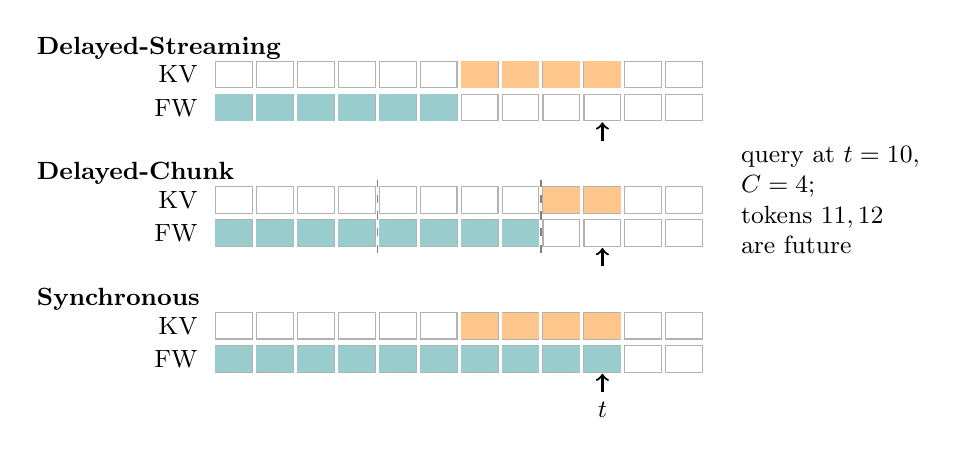
\begin{tikzpicture}[x=0.52cm,y=0.42cm,font=\small]
\def\ctwelveRow#1#2#3#4{%
  \foreach \i in {1,...,12} \draw[gray!60] (\i,#1) rectangle ++(0.9,0.8);
  \foreach \i in {#2} \fill[#4] (\i,#1) rectangle ++(0.9,0.8);
  \node[anchor=east] at (0.8,#1+0.4) {#3};}
\node[anchor=west,font=\small\bfseries] at (-3.6,10.6) {Delayed-Streaming};
\ctwelveRow{9.4}{7,8,9,10}{KV}{orange!45}
\ctwelveRow{8.4}{1,2,3,4,5,6}{FW}{teal!40}
\node[anchor=west,font=\small\bfseries] at (-3.6,6.8) {Delayed-Chunk};
\ctwelveRow{5.6}{9,10}{KV}{orange!45}
\ctwelveRow{4.6}{1,2,3,4,5,6,7,8}{FW}{teal!40}
\node[anchor=west,font=\small\bfseries] at (-3.6,3.0) {Synchronous};
\ctwelveRow{1.8}{7,8,9,10}{KV}{orange!45}
\ctwelveRow{0.8}{1,2,3,4,5,6,7,8,9,10}{FW}{teal!40}
\foreach \y in {0.8,4.6,8.4} \draw[->,thick] (10.45,\y-0.6) -- (10.45,\y-0.05);
\node at (10.45,-0.35) {$t$};
\draw[dashed,gray] (4.95,4.4) -- (4.95,6.6); \draw[dashed,gray] (8.95,4.4) -- (8.95,6.6);
\node[anchor=west,align=left] at (13.6,6.0) {query at $t=10$,\\ $C=4$;\\ tokens $11,12$\\ are future};
\end{tikzpicture}
\caption{Which past tokens each memory holds when the query sits at position $t=10$ with window
(chunk) size $C=4$. Orange: tokens visible to the softmax KV-memory; teal: tokens written into the
delta-rule FW-memory. Dashed lines mark chunk boundaries for Delayed-Chunk.}
\label{fig:c12-hqlt-schemes}
\end{figure}

\Cref{fig:c12-hqlt-schemes} shows the three schemes for one query. In both delayed schemes the
memories \emph{partition} the past: every token is in exactly one of them. Delayed-Streaming
gives the KV-memory a full window of $C$ tokens at every position; Delayed-Chunk gives it
between $1$ and $C$ tokens, depending on where $t$ falls in its chunk. The synchronous scheme
gives up the partition: recent tokens are seen by both, so the FW-memory processes the whole
stream in order with no gap, and the KV-memory adds a precise copy of the last $C$ tokens on top.

\paragraph{Mixing the two reads.} The official layer offers four ways to combine
$\vo^{\mathrm{FW}}_t$ and $\vo^{\mathrm{KV}}_t$:
\begin{align}
  \text{sum:}\quad & \vo_t = \vo^{\mathrm{FW}}_t + \vo^{\mathrm{KV}}_t,\\
  \text{static scalars:}\quad & \vo_t = \lambda^{\mathrm{FW}}\vo^{\mathrm{FW}}_t + \lambda^{\mathrm{KV}}\vo^{\mathrm{KV}}_t,\\
  \text{dynamic scalars:}\quad & \vo_t = \sigmoid(a_t)\,\vo^{\mathrm{FW}}_t + \sigmoid(b_t)\,\vo^{\mathrm{KV}}_t,
     \quad (a_t,b_t) \text{ linear in } \vx_t \text{, per head},\\
  \text{dynamic vector:}\quad & \vo_t = \vg_t\had\vo^{\mathrm{FW}}_t + (\bm1-\vg_t)\had\vo^{\mathrm{KV}}_t,
     \quad \vg_t = \sigmoid(\mW_g\T\vx_t)\in(0,1)^{d_v}. \label{eq:c12-hqlt-gate}
\end{align}
The dynamic vector gate lets each output channel decide, token by token, whether to trust the
precise or the compressed memory. It is the default in the paper's main language-modeling
configs (\cref{sec:c12-hqlt-code}).

\paragraph{Special cases.} If $C\ge T$, the synchronous scheme with sum mixing is exactly a
full softmax attention head plus a DeltaNet head sharing projections. If $C=1$, the KV-memory
returns $\vv_t$ itself and the layer is DeltaNet plus a skip connection on the values. Our NumPy
check verifies the first special case and that Delayed-Streaming equals pure SWA for $t\le C$
(the FW-memory is still empty).

\paragraph{Chunkwise form.} The FW-memory runs in the chunkwise form of the delta rule
(\cref{ch:linear}). We restate it in the form needed here and prove it, because it shows that
Delayed-Chunk costs nothing beyond one chunkwise DeltaNet pass.

\begin{proposition}[Chunkwise delta rule]\label{prop:c12-chunk-delta}
Run the delta rule $\mS_r = \mS_{r-1}(\mI-\beta_r\vk_r\vk_r\T) + \beta_r\vv_r\vk_r\T$ for $r =
1,\dots,n$ inside one chunk, starting from $\mS_0$. Stack the chunk's keys, values and queries as
rows of $\mK\in\R^{n\times d_k}$, $\mV\in\R^{n\times d_v}$, $\mQ\in\R^{n\times d_k}$ and let
$\mD = \diag(\beta_1,\dots,\beta_n)$. Define
\begin{equation}\label{eq:c12-wy}
  \bm\Delta = \big(\mI + \mD\,\mathrm{tril}(\mK\mK\T,-1)\big)^{-1}\mD\,(\mV - \mK\mS_0\T)
  \in\R^{n\times d_v},
\end{equation}
where $\mathrm{tril}(\cdot,-1)$ keeps the strictly lower triangle. Then $\mS_n = \mS_0 +
\bm\Delta\T\mK$, and the outputs $\vo_r = \mS_r\vq_r$ are the rows of $\mQ\mS_0\T +
\mathrm{tril}(\mQ\mK\T)\bm\Delta$.
\end{proposition}
\begin{proof}
Write one step as $\mS_r = \mS_{r-1} + \bm\delta_r\vk_r\T$ with $\bm\delta_r =
\beta_r(\vv_r - \mS_{r-1}\vk_r)$. Unrolling, $\mS_r = \mS_0 + \sum_{j\le r}\bm\delta_j\vk_j\T$,
hence $\mS_{r-1}\vk_r = \mS_0\vk_r + \sum_{j<r}\bm\delta_j(\vk_j\T\vk_r)$. Substituting into the
definition of $\bm\delta_r$ and moving the sum to the left,
\[
  \bm\delta_r + \beta_r\sum_{j<r}(\vk_r\T\vk_j)\,\bm\delta_j = \beta_r(\vv_r - \mS_0\vk_r),
\]
which is row $r$ of $(\mI + \mD\,\mathrm{tril}(\mK\mK\T,-1))\bm\Delta = \mD(\mV - \mK\mS_0\T)$
with $\bm\delta_r\T$ the rows of $\bm\Delta$. The matrix on the left is unit lower triangular,
hence invertible, which gives \eqref{eq:c12-wy}. Then $\mS_n = \mS_0 + \sum_j\bm\delta_j\vk_j\T
= \mS_0 + \bm\Delta\T\mK$, and $\mS_r\vq_r = \mS_0\vq_r + \sum_{j\le r}(\vq_r\T\vk_j)\bm\delta_j$
is row $r$ of $\mQ\mS_0\T + \mathrm{tril}(\mQ\mK\T)\bm\Delta$.
\end{proof}

The output has an \emph{inter-chunk} part $\mQ\mS_0\T$ (read the state left by earlier chunks)
and an \emph{intra-chunk} part $\mathrm{tril}(\mQ\mK\T)\bm\Delta$. Delayed-Chunk HQLT keeps the
inter-chunk part of the FW-memory and \emph{replaces the intra-chunk part by causal softmax
attention restricted to the chunk}. So one layer computes, for chunk $i$,
\begin{equation}\label{eq:c12-delayed-chunk}
  \mO_{[i]} = \underbrace{\softmax\!\Big(\tfrac{\tilde\mQ_{[i]}\tilde\mK_{[i]}\T}{\sqrt{d_k}} + \mM\Big)\mV_{[i]}}_{\text{KV-memory, intra-chunk}}
  \;\oplus\; \underbrace{\hat\mQ_{[i]}\mS_{[i]}\T}_{\text{FW-memory, inter-chunk}},\qquad
  \mS_{[i+1]} = \mS_{[i]} + \bm\Delta_{[i]}\T\hat\mK_{[i]},
\end{equation}
with $\oplus$ the chosen mixing. In words: the chunkwise algorithm of a linear Transformer
already splits the work into ``within the chunk'' and ``across chunks''; Delayed-Chunk HQLT uses
the expensive exact mechanism where it is cheap (inside a chunk) and the compressed one where it
must be cheap (across chunks). The synchronous scheme instead keeps both parts of the FW output
and adds a sliding-window attention on top.

\subsection{Algorithms and complexity}

\Cref{alg:c12-hqlt} gives the synchronous scheme for decoding, the variant used at inference
in the official code. Prefill uses the same equations in parallel form: FlashAttention with a
window of $C$ for the KV-memory and the chunkwise delta rule of
\cref{prop:c12-chunk-delta} for the FW-memory.

\begin{algorithm}[t]
\caption{One decoding step of a synchronous HQLT head with dynamic vector mixing.}
\label{alg:c12-hqlt}
\begin{algorithmic}[1]
\Require input $\vx_t$; ring buffer $\mathcal{B}$ of the last $C-1$ pairs $(\tilde\vk_s,\vv_s)$; FW state $\mS$
\State $\vq,\vk \gets \mW_Q\T\vx_t, \mW_K\T\vx_t$;\quad $\vv\gets\SiLU(\mW_V\T\vx_t)$;\quad $\beta\gets\sigmoid(\vw_\beta\T\vx_t)$
\LineComment{KV-memory: exact recall of the last $C$ tokens}
\State $\tilde\vq,\tilde\vk \gets \mathrm{RoPE}_t(\vq), \mathrm{RoPE}_t(\vk)$; append $(\tilde\vk,\vv)$ to $\mathcal{B}$; drop the oldest pair if $\abs{\mathcal{B}}>C$
\State $\vo^{\mathrm{KV}} \gets \sum_{(\vk',\vv')\in\mathcal{B}}\softmax(\tilde\vq\T\vk'/\sqrt{d_k})\,\vv'$
\LineComment{FW-memory: delta-rule write and read}
\State $\hat\vq,\hat\vk \gets \SiLU(\vq)/\norm{\SiLU(\vq)},\ \SiLU(\vk)/\norm{\SiLU(\vk)}$
\State $\mS \gets \mS - \beta\,(\mS\hat\vk - \vv)\hat\vk\T$ \Comment{$=\mS(\mI-\beta\hat\vk\hat\vk\T)+\beta\vv\hat\vk\T$}
\State $\vo^{\mathrm{FW}} \gets \mS\hat\vq$
\State $\vg\gets\sigmoid(\mW_g\T\vx_t)$;\quad $\vo \gets \vg\had\vo^{\mathrm{FW}} + (\bm1-\vg)\had\vo^{\mathrm{KV}}$
\State \Return $\mW_O\,\RMSNorm(\vo)$ \Comment{heads concatenated before $\mW_O$}
\end{algorithmic}
\end{algorithm}

\paragraph{Cost.} Per head and token, decoding costs $\bigO(C(d_k+d_v))$ for the window and
$\bigO(d_kd_v)$ for the delta rule; the memory is $C(d_k+d_v) + d_kd_v$ numbers, \emph{constant}
in the sequence length. Prefill costs $\bigO(TC(d_k+d_v))$ for windowed attention plus
$\bigO(TCd_k + Td_kd_v)$ for the chunkwise delta rule, i.e.\ linear in $T$. For
Delayed-Streaming decoding the pair evicted from the ring buffer is exactly the one written into
$\mS$, so the two memories form a single pipeline: tokens flow through the exact buffer and then
into the fast weights.

\subsection{Implementation walkthrough}\label{sec:c12-hqlt-code}

The official code (\repo{kazuki-irie__hybrid-memory}) is a fork of \fla{} and its training
framework \textsf{flame}, plus two experiment folders (synthetic algorithmic tasks and
reinforcement learning).

\begin{implnote}[title={In the code: files and the confusing mode names}]
The layer is \code{HybridQLT} in \repofile{repos/kazuki-irie__hybrid-memory/fla/fla/layers/hybrid_qlt.py};
the model wrapper is \code{HybridQLTBlock} in \repofile{fla/fla/models/hybrid_qlt/modeling_hybrid_qlt.py}.
The scheme is selected by \code{attn_mode}, whose names do not match the paper. The repository's
\repofile{fla/README.md} gives the mapping:
\begin{center}\small
\begin{tabular}{@{}ll@{}}
\toprule
\code{attn_mode} & paper scheme \\
\midrule
\code{sync_chunk} & Synchronous (FW-memory = DeltaNet) \\
\code{chunk} & Delayed-Chunk \\
\code{delayed} & Delayed-Streaming \\
\code{sync_chunk_linear} & Synchronous with plain linear attention as FW-memory \\
\bottomrule
\end{tabular}
\end{center}
\code{HybridQLTBlock} can also place ordinary attention layers at chosen indices
(\code{config.attn['layers']}), so HQLT layers can themselves be interleaved serially with full
attention. A file comment notes that context carry-over between batches is not implemented for
Delayed-Chunk ``as Synchronous HQLT is a better choice regardless''.
\end{implnote}

\begin{implnote}[title={In the code: one set of projections, two branches}]
\code{forward} computes \code{q_proj}, \code{k_proj}, \code{v_proj} once (the language-model
configs set \texttt{use\_short\_conv: false}, in which case the value is passed through
\code{F.silu}). The KV branch applies \code{self.rotary} (enabled by
\code{use_local_pos_encoding}) and calls \texttt{flash\_attn\_func(..., causal=True, window\_size=(self.chunk\_size-1, 0))}: the window is the current token plus $C-1$ previous ones,
so the window size and the chunk size are the same hyperparameter \code{chunk_size}. The FW
branch applies \code{F.silu} to \code{q} and \code{k} and calls \texttt{chunk\_delta\_rule(..., use\_qk\_l2norm\_in\_kernel=True)}, which normalizes inside the kernel. At inference the cache
(\repofile{fla/fla/models/utils.py}, \code{Cache.update} with \code{use_special=True}) keeps only
the last \code{window_size} keys and values, so the KV-memory really is bounded.
\end{implnote}

\Cref{lst:c12-hqlt-delay} shows how Delayed-Streaming is implemented during training: the FW
branch sees the key and value sequences shifted right by $C$ positions, padded with zeros.

\begin{lstlisting}[caption={Excerpt from \texttt{repos/\allowbreak kazuki-irie\_\_hybrid-memory/\allowbreak fla/\allowbreak fla/\allowbreak layers/\allowbreak hybrid\_qlt.py} (Delayed-Streaming, no cache).},label={lst:c12-hqlt-delay}]
            else:
                # append k and v zeros of length chunk
                k_padd_zeros = torch.zeros(
                    [batch_size, window_size, self.num_heads, self.head_k_dim],
                    dtype=k.dtype, device=k.device)
                v_padd_zeros = torch.zeros(
                    [batch_size, window_size, self.num_heads, self.head_v_dim],
                    dtype=v.dtype, device=v.device)
                k_fw = torch.cat([k_padd_zeros, F.silu(k[:, :-window_size])], dim=1)[:, :q_len]
                v_fw = torch.cat([v_padd_zeros, v[:, :-window_size]], dim=1)[:, :q_len]

            o_fw, recurrent_state = chunk_delta_rule(
                q=q,
                k=k_fw,
                v=v_fw,
                beta=beta,
                initial_state=recurrent_state,
                output_final_state=use_cache,
                cu_seqlens=cu_seqlens,
                use_qk_l2norm_in_kernel=True if self.qk_norm == 'l2' else False
            )
\end{lstlisting}

Two details are worth checking by hand. First, a zero key is a no-op write: $\mathrm{SiLU}(0) =
0$, the in-kernel normalization maps $\bm0$ to $\bm0$, and $\mS(\mI - \beta\bm0\bm0\T) +
\beta\bm0\bm0\T = \mS$, so the padding implements ``the FW-memory is empty for $t\le C$''. Our
check confirms that the zero-padded shift equals the definition exactly. Second, \code{beta} is
\emph{not} shifted: the write strength applied to token $t-C$ is computed from the input at
time $t$. This is why \eqref{eq:c12-hqlt-fw} carries two time indices.

\begin{implnote}[title={In the code: the Delayed-Chunk kernel}]
For \code{attn_mode="chunk"} the layer calls \code{chunk_hybrid_softmax_delta_rule} from
\repofile{fla/fla/ops/hybrid_qlt/chunk.py}. Its forward pass runs the WY preparation
(\code{prepare_wy_repr_fwd}, the matrix inverse of \eqref{eq:c12-wy}), propagates chunk states
(\code{chunk_gated_delta_rule_fwd_h} with no gate), and then calls
\code{chunk_no_local_fwd_o}, which computes only the inter-chunk term $\hat\mQ_{[i]}\mS_{[i]}\T$,
and \code{parallel_chunk_only_attn_fwd}, a FlashAttention-style kernel whose attention never
crosses a chunk boundary. The test file \repofile{fla/tests/ops/test_hybrid_softmax_delta.py}
contains naive references (\code{naive_local_attn}, \code{naive_non_local_deltanet}) that make
the decomposition of \eqref{eq:c12-delayed-chunk} explicit.
\end{implnote}

The mixing step at the end of \code{forward} is short enough to quote in full:

\begin{lstlisting}[caption={Excerpt from \texttt{repos/\allowbreak kazuki-irie\_\_hybrid-memory/\allowbreak fla/\allowbreak fla/\allowbreak layers/\allowbreak hybrid\_qlt.py} (mixing the two memories).},label={lst:c12-hqlt-mix}]
        if self.use_memory_gate:
            mg = rearrange(self.memory_gate_proj(hidden_states), '... (h d) -> ... h d', d=self.head_v_dim * self.num_gates).sigmoid()
            if self.num_gates == 1:
                o = mg * o_fw + (1 - mg) * o_kv
            else:
                assert self.num_gates == 2
                mg_fw, mg_kv = torch.split(mg, (self.head_v_dim, self.head_v_dim), -1)
                o = mg_fw * o_fw + mg_kv * o_kv
        elif self.use_memory_dynamic_scaler:
            mg = self.memory_mixer(hidden_states).sigmoid()
            mg_fw, mg_kv = torch.split(mg, (self.num_heads, self.num_heads), -1)
            o = mg_fw.unsqueeze(-1) * o_fw + mg_kv.unsqueeze(-1) * o_kv
        elif self.use_memory_scaler:
            o = self.fw_scale * o_fw + self.kv_scale * o_kv
        else:
            o = o_fw + o_kv
\end{lstlisting}

\begin{implnote}[title={In the code: configs}]
\repofile{repos/kazuki-irie__hybrid-memory/language_modeling/configs/} contains one JSON file per
model in the paper. The file names encode scheme, chunk size and mixing, e.g.\
\code{sync_hqlt_ch64_dynamic-vector-mixing_noconv_340M.json}. That config sets
\texttt{hidden\_size: 1024}, \texttt{num\_hidden\_layers: 24}, \texttt{num\_heads: 8} (head dimension
$128$), \texttt{chunk\_size: 64}, \texttt{use\_local\_pos\_encoding: true} and \texttt{use\_memory\_gate: true} (dynamic vector mixing, \eqref{eq:c12-hqlt-gate}). Sum and dynamic-scalar mixing are the
\code{sum-mixing} and \code{dynamic-scalar-mixing} files (\texttt{use\_memory\_dynamic\_scaler: true}); ablations vary the chunk size from 64 to 1024 and drop RoPE (\code{NoPos}). Baselines
(Transformer, DeltaNet, Mamba, Mamba-2, GLA, HGRN-2, Samba, \dots) live in the same folder. The
README's training command uses AdamW with learning rate $10^{-3}$, cosine decay with 1024 warmup
steps and sequence length 2048 on FineWeb-Edu (2240 for the 1.3B models). The synthetic parity
config (\repofile{synthetic_algorithmic/experiments/parity_sync_hqlt_net.yaml}) uses 2 layers of
width 128, \texttt{chunk\_size: 8}, \texttt{allow\_neg\_eigval: true} (which doubles $\beta$, see
\cref{sec:c12-olmo}), training lengths 3--40 and test lengths 40--256: it tests length
generalization of state tracking.
\end{implnote}

\subsection{Reference implementation}

\Cref{lst:c12-hqlt-ref} implements the three schemes for one head with dynamic vector mixing,
token by token for clarity (RoPE and the output norm are omitted). It is the recurrent form; the
NumPy check compares it with the chunkwise form.

\begin{lstlisting}[caption={Reference implementation (ours): quadratic-linear blending with the three schemes, one head.},label={lst:c12-hqlt-ref}]
import torch, torch.nn as nn, torch.nn.functional as F

class QuadLinearBlend(nn.Module):
    """Softmax KV-memory over C tokens + delta-rule FW-memory; scheme in {sync, stream, chunk}."""
    def __init__(self, d, dk, dv, C, scheme="sync"):
        super().__init__()
        self.q, self.k = nn.Linear(d, dk, bias=False), nn.Linear(d, dk, bias=False)
        self.v, self.b = nn.Linear(d, dv, bias=False), nn.Linear(d, 1, bias=False)
        self.g = nn.Linear(d, dv, bias=False)             # dynamic vector mixing gate
        self.C, self.scheme = C, scheme

    def forward(self, x):                                  # x: (T, d), one sequence
        T, C, dk = x.shape[0], self.C, self.q.out_features
        q, k, v = self.q(x), self.k(x), F.silu(self.v(x))  # shared projections
        beta = torch.sigmoid(self.b(x)).squeeze(-1)
        qf, kf = F.normalize(F.silu(q), dim=-1), F.normalize(F.silu(k), dim=-1)
        S = x.new_zeros(v.shape[1], dk)
        o_kv, o_fw = [], []
        for t in range(T):
            if self.scheme == "chunk":
                lo = (t // C) * C                          # attend inside the chunk only
                if t % C == 0:
                    S0 = S.clone()                         # FW state left by earlier chunks
            else:
                lo = max(0, t - C + 1)                     # sliding window of C tokens
            a = torch.softmax(q[t] @ k[lo:t + 1].T / dk ** 0.5, dim=-1)
            o_kv.append(a @ v[lo:t + 1])
            if self.scheme == "sync":                      # token t enters both memories now
                S = S - beta[t] * torch.outer(S @ kf[t] - v[t], kf[t])
                o_fw.append(S @ qf[t])
            elif self.scheme == "stream":                  # token t-C leaves window -> FW
                if t >= C:
                    s = t - C
                    S = S - beta[t] * torch.outer(S @ kf[s] - v[s], kf[s])
                o_fw.append(S @ qf[t])
            else:                                          # "chunk": inter-chunk read only
                o_fw.append(S0 @ qf[t])
                S = S - beta[t] * torch.outer(S @ kf[t] - v[t], kf[t])
        o_kv, o_fw = torch.stack(o_kv), torch.stack(o_fw)
        g = torch.sigmoid(self.g(x))
        return g * o_fw + (1 - g) * o_kv
\end{lstlisting}

\paragraph{Numerical check.} In NumPy (\texttt{check\_hqlt.py}, $T=23$, $d_k=4$, $d_v=3$, $C=5$,
so the last chunk is partial) we computed Delayed-Chunk twice, once token by token as in
\cref{lst:c12-hqlt-ref} and once in the chunkwise form \eqref{eq:c12-delayed-chunk} with the WY
matrix of \eqref{eq:c12-wy}. The maximum difference was $6.7\times10^{-16}$. The synchronous FW
output in chunkwise form (\cref{prop:c12-chunk-delta}) matched the recurrence to
$5.6\times10^{-16}$. We also confirmed the zero-padded shift of \cref{lst:c12-hqlt-delay}, the
partition property for $t\le C$, and the $C\ge T$ special case.

\begin{results}
\textbf{Source:} \repofile{repos/kazuki-irie__hybrid-memory/README.md} and the sub-READMEs. The
repository contains no result numbers; it maps the code to the paper's tables (language modeling:
Tables~1 and~3; synthetic algorithmic tasks: Table~2; reinforcement learning: Figure~2) and
provides configs for 340M- and 1B/1.3B-scale models. Qualitatively, the paper reports that the
two memories have complementary strengths (precise retrieval versus long sequences and expressive
computation), that a well-designed hybrid overcomes the limitations of its components, and that
the synthetic tasks single out the benefit of certain blending schemes over others; a code
comment in \code{hybrid_qlt.py} states that the synchronous scheme ``is a better choice
regardless''. See the paper for numbers.
\end{results}

\subsection{Discussion}

\paragraph{Why synchronous wins (an interpretation).} In both delayed schemes the FW-memory
never sees the most recent $C$ tokens, so any computation that needs the full stream in order
(parity, modular arithmetic, tracking a state machine) must be finished by the windowed softmax,
which is poor at it. In the synchronous scheme the delta-rule memory processes every token
immediately, keeping its expressivity, while the KV-memory adds precise recall of the recent
window. The price is that recent tokens are stored twice. This reading is ours; the paper's
synthetic tasks are designed to test exactly this difference.

\paragraph{Limits.} The KV-memory is a window of $C$ tokens (64 in the main configs). Beyond the
window, recall is again bounded by \cref{prop:c12-capacity}: HQLT does not give exact recall of
a fact from thousands of tokens ago. A full model therefore still benefits from a few
full-attention layers, which \code{HybridQLTBlock} supports.

\paragraph{Relations.} Delayed-Streaming is the same idea as RATTENTION's residual linear
attention over tokens that left the window (\cref{ch:sparse}) and as B'MOJO's eidetic-plus-fading
memory \citep{c12-zancato2024bmojo}; the synchronous scheme is Samba's serial SWA-plus-SSM pairing
moved inside one layer. The survey highlights HQLT as a fixed-budget precursor of HAM, which
replaces the fixed window by a KV cache that admits only the tokens the recurrent state predicts
poorly (\cref{ch:routing}).
% ===========================================================================================
\section{Hymba: parallel attention and SSM heads}\label{sec:c12-hymba}

\subsection{Motivation}

Hymba \citep{dong2025hymba} targets small language models (about 1.5B parameters), where every
layer is precious and a serial hybrid would leave most layers without precise recall. Its
answer is the \emph{hybrid-head} layer: inside every layer, attention heads and SSM heads read
the same input in parallel. In the README's words, ``attention heads provide high-resolution
recall, while SSM heads enable efficient context summarization''. Three further ideas shrink the
KV cache and fix a weakness of softmax attention: most layers use sliding-window attention with
only a few full-attention layers; adjacent layers share keys and values; and a set of learnable
\emph{meta tokens} is prepended to every input.

\begin{taxonomy}
Hymba is not listed in the survey's Table~I; Section~V-A of \citet{zhoubian2026memory} groups it
with Falcon-H1 as a hybrid-head model in which ``attention and recurrent/state-space memory can
be combined \dots\ within the same layer'' with a fixed, architecture-determined allocation. In
the taxonomy's terms: the KV caches and SSM states are \textbf{implicit}, \textbf{online} memory;
the sliding-window caches are \textbf{short-term} and the SSM state and the few global layers
carry \textbf{long-term} context. The meta tokens are learned parameters fixed after training,
i.e.\ a small \textbf{offline} memory (\cref{cor:c12-meta}). Update rules: state transitions
(SSM), admission and eviction (sliding window).
\end{taxonomy}

\subsection{Formulation}

\paragraph{The hybrid-head layer.} Let $\vx_t\in\R^d$ be the normalized input and $d_{\mathrm{in}}
= e\,d$ the inner width ($e = 2$, the Mamba expansion). One input projection produces everything
both branches need,
\begin{equation}\label{eq:c12-hymba-in}
  [\,\vq_t;\ \vk_t;\ \vv_t;\ \vu_t;\ \vz_t\,] = \mW_{\mathrm{in}}\vx_t + \vb_{\mathrm{in}},
  \qquad \vq_t,\vu_t,\vz_t\in\R^{d_{\mathrm{in}}},\ \vk_t,\vv_t\in\R^{H_{kv}d_h},
\end{equation}
where $\vq,\vk,\vv$ feed $H$ attention heads of size $d_h = d_{\mathrm{in}}/H$ with grouped
keys/values ($H_{kv}<H$), $\vu$ is the SSM input and $\vz$ its output gate. The attention branch
returns $\vy^{\mathrm{att}}_t\in\R^{d_{\mathrm{in}}}$. The SSM branch is a Mamba (selective
scan) layer: after a short causal convolution and $\SiLU$, it computes per channel $c$ and state
index $n$
\begin{equation}\label{eq:c12-mamba1}
  h_{t,cn} = e^{\Delta_{t,c}A_{cn}}\,h_{t-1,cn} + \Delta_{t,c}\,B_{t,n}\,u_{t,c},\qquad
  y^{\mathrm{ssm}}_{t,c} = \Big(\sum_n C_{t,n}h_{t,cn} + D_cu_{t,c}\Big)\SiLU(z_{t,c}),
\end{equation}
with $A_{cn}<0$ learned and $\Delta_t, B_t, C_t$ computed from $\vu_t$ (\cref{ch:linear}).
For each channel $c$ this is the generic recurrence \eqref{eq:c12-generic-rec} with a diagonal
transition. Finally the branches are fused by averaging their separately normalized outputs,
\begin{equation}\label{eq:c12-hymba-fuse}
  \vy_t = \mW_{\mathrm{out}}\,\tfrac12\big(\vbeta_1\had\RMSNorm(\vy^{\mathrm{att}}_t) +
  \vbeta_2\had\RMSNorm(\vy^{\mathrm{ssm}}_t)\big),
\end{equation}
where $\vbeta_1,\vbeta_2\in\R^{d_{\mathrm{in}}}$ are learnable per-channel scales (in the code, the
weights of the two RMSNorms). The normalization matters: the attention output is a convex
combination of values while the SSM output is an unnormalized sum, so their scales can differ
by orders of magnitude; normalizing first lets $\vbeta_1,\vbeta_2$ set the balance.

\paragraph{Meta tokens.} Let $\bm{R}\in\R^{M\times d}$ be learned vectors. Hymba runs the network on
$[\bm{R};\mX]$ and drops the first $M$ outputs. The motivation is the ``forced-to-attend'' problem:
softmax weights must sum to one, so a head with nothing relevant to read still has to put its
mass somewhere, typically on the first tokens (``attention sinks'',
\citealp{xiao2023streamingllm}). Meta tokens give it learned places to do so and can store
information useful for every input. Causality makes them cheap.

\begin{proposition}[Meta tokens do not depend on the prompt]\label{prop:c12-meta}
Suppose every sub-layer is causal, i.e.\ its output at position $m$ depends only on its inputs at
positions $\le m$ (causal or windowed attention, causal convolution, SSM scans, and position-wise
norms and MLPs all qualify). Then for every layer $\ell$ and every $m\le M$, the hidden state
$\vh^{(\ell)}_m$ of the input $[\bm{R};\mX]$ is a function of $\bm{R}$ and the parameters only.
\end{proposition}
\begin{proof}
Induction on $\ell$. At $\ell = 0$ the first $M$ rows are the rows of $\bm{R}$. If the claim holds at
layer $\ell$, the output of layer $\ell+1$ at position $m\le M$ depends only on layer-$\ell$
states at positions $\le m\le M$, which by hypothesis do not involve $\mX$.
\end{proof}

\begin{corollary}\label{cor:c12-meta}
The keys and values of the meta tokens in every attention layer, and the SSM state after the
$M$-th position, are constants. They can be computed once and stored: the meta tokens are
equivalent to a learned prefix of the KV cache plus a learned initial SSM state $\vh_0$.
\end{corollary}

Our NumPy check (\texttt{check\_mixer.py}) builds two hybrid-head layers with a meta prefix and a
sliding window, changes the prompt (content and length), and confirms that the meta positions'
hidden states, keys, values and SSM state are unchanged; it also confirms that scanning $\mX$ from
the cached meta state reproduces the scan over $[\bm{R};\mX]$ exactly.

\paragraph{Local and global attention.} Most Hymba layers use a sliding window of $w$ tokens, but
the meta tokens stay visible in every window. The attention mask at query $i$ and key $j$ is
\begin{equation}\label{eq:c12-hymba-mask}
  \mathrm{allowed}(i,j) = [\,j\le i\,]\wedge\big([\,i-j\le w\,]\vee[\,j<M\,]\big),
\end{equation}
shown in \cref{fig:c12-hymba-mask}. A few layers use full attention. Since every layer also has
SSM heads, the long-range path through the network never breaks.

\begin{figure}[t]
\centering
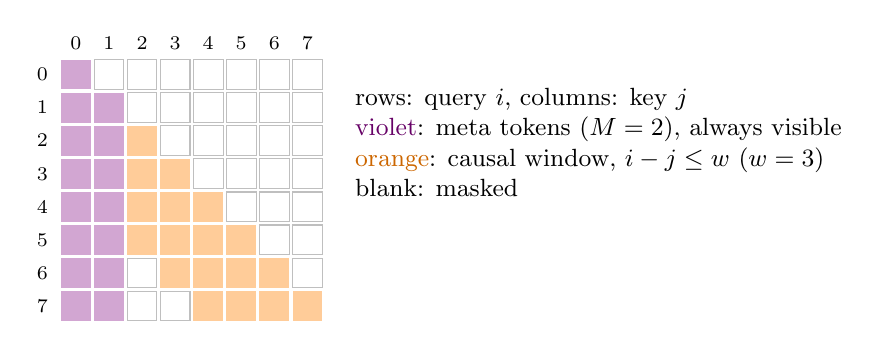
\begin{tikzpicture}[x=0.42cm,y=0.42cm,font=\scriptsize]
\foreach \i in {0,...,7} {
  \foreach \j in {0,...,7} {
    \pgfmathtruncatemacro{\ok}{((\j<=\i) && ((\i-\j<=3) || (\j<2))) ? 1 : 0}
    \ifnum\ok=1
      \ifnum\j<2 \fill[violet!35] (\j,-\i) rectangle ++(0.9,-0.9);
      \else \fill[orange!40] (\j,-\i) rectangle ++(0.9,-0.9); \fi
    \else \draw[gray!50] (\j,-\i) rectangle ++(0.9,-0.9); \fi
  }
  \node[anchor=east] at (-0.1,-\i-0.45) {\i};
  \node at (\i+0.45,0.5) {\i};
}
\node[anchor=west,align=left,font=\small] at (8.6,-2.5) {rows: query $i$, columns: key $j$\\
\textcolor{violet!80!black}{violet}: meta tokens ($M=2$), always visible\\
\textcolor{orange!80!black}{orange}: causal window, $i-j\le w$ ($w=3$)\\ blank: masked};
\end{tikzpicture}
\caption{Hymba's sliding-window mask with meta tokens, as computed by the predicate in
\texttt{barebones\_hymba\_block.py} for $w=3$ and two meta tokens. Each query sees the meta
tokens plus the last $w+1$ positions (itself included).}
\label{fig:c12-hymba-mask}
\end{figure}

\paragraph{Cross-layer KV sharing.} If a group of $g$ consecutive layers uses the keys and values
computed by the first layer of the group (the other layers only compute queries), the group
stores one KV cache instead of $g$. Combining the pieces, for $L_g$ global and $L_\ell$ local
attention layers with $H_{kv}$ key--value heads of size $d_h$, the KV cache after $T$ tokens is
\begin{equation}\label{eq:c12-hymba-cache}
  \frac{2H_{kv}d_h}{g}\Big(L_g\,(M+T) + L_\ell\,\big(M+\min(T,w+1)\big)\Big),
\end{equation}
plus a constant SSM state of $d_{\mathrm{in}}\times N$ numbers per layer. Only the global term
grows with $T$.

\begin{example}[Cache arithmetic for the barebones config]\label{ex:c12-hymba-cache}
The barebones \code{HymbaConfig} (below) has 32 layers of which 5 are global, $H_{kv}=2$, $d_h =
256$, $M = 256$ and $w = 2048$, and the barebones code does not share KV ($g=1$). One layer stores
$2\cdot2\cdot256 = 1{,}024$ numbers per cached token. At $T = 8{,}192$,
\eqref{eq:c12-hymba-cache} gives $1{,}024\,(5\cdot8{,}448 + 27\cdot2{,}305)\approx1.07\times10^8$
numbers, against $1{,}024\cdot32\cdot8{,}448\approx2.77\times10^8$ for 32 global layers (our
arithmetic). KV sharing with $g = 2$ would halve the first number again. The SSM state adds
$3{,}072\cdot16 = 49{,}152$ numbers per layer.
\end{example}

\subsection{Algorithm}

\begin{algorithm}[t]
\caption{Forward pass of a Hymba-style hybrid-head layer (prefill; one sequence).}
\label{alg:c12-hymba}
\begin{algorithmic}[1]
\Require $\mX\in\R^{T\times d}$ (meta tokens already prepended), window $w$ or \textsc{global}
\State $[\mQ;\mK;\mV;\mU;\mZ] \gets \mX\mW_{\mathrm{in}}\T + \vb_{\mathrm{in}}$ \Comment{one fused projection, \eqref{eq:c12-hymba-in}}
\State $\mY^{\mathrm{att}} \gets \mathrm{GQA}(\mQ,\mK,\mV)$, RoPE, mask \eqref{eq:c12-hymba-mask} \Comment{$\bigO(T\min(T,w+M)d_{\mathrm{in}})$}
\State $\mU \gets \SiLU(\mathrm{conv1d}(\mU))$;\ \ $(\bm\Delta,\mB,\mC) \gets$ projections of $\mU$
\State $\mY^{\mathrm{ssm}} \gets$ selective scan \eqref{eq:c12-mamba1} gated by $\SiLU(\mZ)$ \Comment{$\bigO(Td_{\mathrm{in}}N)$}
\State \Return $\tfrac12\big(\RMSNorm(\mY^{\mathrm{att}}) + \RMSNorm(\mY^{\mathrm{ssm}})\big)\mW_{\mathrm{out}}\T$
\end{algorithmic}
\end{algorithm}

During decoding the attention branch reads at most $M + w + 1$ cached pairs in local layers and
$M+t$ in global ones; the SSM branch updates a $d_{\mathrm{in}}\times N$ state. Time per token is
therefore $\bigO((M+w)d_{\mathrm{in}})$ in local layers, independent of $t$.

\subsection{Implementation walkthrough}

The mirror (\repo{NVlabs__hymba}) contains a chat script, an evaluation harness and a minimal
``barebones'' implementation; the full model code is on Hugging Face (\code{modeling_hymba.py},
not mirrored). The barebones README lists what it includes (parallel fused attention and Mamba
heads, meta tokens with SWA, mix of local and global attention) and what it leaves out (cache
management for generation, cross-layer KV reuse).

\begin{implnote}[title={In the code: one projection, split five ways}]
\code{HymbaBlock} in \repofile{repos/NVlabs__hymba/barebones_hymba/barebones_hymba_block.py}
sets \texttt{intermediate\_size = mamba\_expand * hidden\_size} and
\texttt{attention\_head\_size = intermediate\_size / num\_attention\_heads}. With the barebones config
($d = 1536$, expansion 2, 12 heads, 2 KV heads) this gives $d_{\mathrm{in}} = 3072$ and $d_h=256$.
\code{latent_dim} adds the SSM input ($3072$), the queries ($3072$) and keys plus values
($2\cdot2\cdot256 = 1024$), so \code{in_proj} is \texttt{nn.Linear(1536, 7168 + 3072)} with bias,
the last $3072$ outputs being the gate $\vz$. \code{forward} splits the projection with
\code{tensor_split} in the order (query, key, value, SSM input) $|$ gate, runs
\code{self.self_attn} and \code{self.mamba}, and asserts that both outputs have the same shape.
\end{implnote}

\begin{lstlisting}[caption={Excerpt from \texttt{repos/\allowbreak NVlabs\_\_hymba/\allowbreak barebones\_hymba/\allowbreak barebones\_hymba\_block.py} (end of \texttt{HymbaBlock.forward}).},label={lst:c12-hymba-fuse}]
        attn_outputs = self.self_attn(
            query_states=query_states,
            key_states=key_states,
            value_states=value_states
        )

        mamba_outputs = self.mamba(hidden_states=hidden_states, gate=gate)


        assert attn_outputs.shape == mamba_outputs.shape
        hidden_states = (self.pre_avg_layernorm1(attn_outputs) + self.pre_avg_layernorm2(mamba_outputs)) / 2
        contextualized_states = self.out_proj(hidden_states)
\end{lstlisting}

\begin{implnote}[title={In the code: the SSM branch}]
\code{MambaBranch} applies \texttt{causal\_conv1d\_fn(..., activation="silu")}, projects to
$(\Delta,B,C)$ with \code{x_proj} (time-step rank 8, state size 16), applies separate RMSNorms to
$\Delta$, $B$ and $C$ (\code{dt_layernorm}, \code{B_layernorm}, \code{C_layernorm}), and calls
\code{selective_scan_fn} from \textsf{mamba\_ssm} with \code{z=gate}, \code{delta_softplus=True}
and the bias of \code{dt_proj} passed separately as \code{delta_bias}. $A$ is initialized as
\texttt{A = arange(1, N+1)} for every channel and stored as its logarithm \code{A_log}; the
scan uses $A=-\exp(\log A)$, so all decays $e^{\Delta A}$ lie in $(0,1)$.
\end{implnote}

\begin{lstlisting}[caption={Excerpt from \texttt{repos/\allowbreak NVlabs\_\_hymba/\allowbreak barebones\_hymba/\allowbreak barebones\_hymba\_block.py} (\texttt{AttentionBranch.\_\_init\_\_}, mask construction).},label={lst:c12-hymba-mask}]
            def sliding_window(b, h, q_idx, kv_idx):
                return q_idx - kv_idx <= self.attention_window_size

            def causal_mask(b, h, q_idx, kv_idx):
                return q_idx >= kv_idx
            attn_mask = and_masks(causal_mask, sliding_window)
       
            def prefix_mask(b, h, q_idx, kv_idx):
                return kv_idx < self.num_meta_tokens
            register_mask = and_masks(causal_mask, prefix_mask)

            self.attn_mask = or_masks(attn_mask, register_mask) # real mask we use 
\end{lstlisting}

\begin{implnote}[title={In the code: masks, configs and caveats}]
The mask of \cref{lst:c12-hymba-mask} is compiled into a FlexAttention block mask (PyTorch
$\ge2.5$). With \code{modify_attention_mask=False} the code falls back to
\texttt{flash\_attn\_func(..., causal=True, window\_size=(w, w))}, which drops the meta-token
exception. Note an off-by-one between the comment above the mask (drawn with $w$ visible
positions) and the predicate \texttt{q\_idx - kv\_idx <= w}, which admits $w+1$ positions including
the query itself (\cref{fig:c12-hymba-mask} shows the predicate). The test model in
\repofile{barebones_hymba/test_barebones_hymba.py} has \texttt{num\_layers = 32},
\texttt{global\_layer\_list = [5,11,18,25,31]}, \texttt{hidden\_size = 1536},
\texttt{num\_meta\_tokens = 256}, \texttt{attention\_window\_size = 2048}, \texttt{ssm\_state\_size = 16},
\texttt{intermediate\_size = 4608} for the MLP, and RoPE base $10^4$; \code{SimplifiedHymba}
prepends \code{self.meta_token} to the batch and strips the first \code{num_meta_tokens} outputs.
The top-level README warns that generation currently needs batch size 1 because padding is not
fully supported together with meta tokens and SWA.
\end{implnote}

\subsection{Reference implementation}

\Cref{lst:c12-parallel} is a parallel-head mixer that covers both Hymba and Falcon-H1
(\cref{sec:c12-falcon}). The SSM is passed in as any causal module, so the listing stays short;
any recurrence from \cref{ch:linear} can be plugged in.

\begin{lstlisting}[caption={Reference implementation (ours): a parallel-head hybrid mixer (Hymba / Falcon-H1 style).},label={lst:c12-parallel}]
import torch, torch.nn as nn

class ParallelHybridMixer(nn.Module):
    """fuse="mean_norm": Hymba (average of RMS-normalized branches, one projection).
       fuse="concat":    Falcon-H1 (concatenate branches, one projection)."""
    def __init__(self, d, n_heads, n_kv, d_head, d_ssm, ssm, window=None, n_meta=0,
                 fuse="mean_norm"):
        super().__init__()
        self.h, self.hkv, self.dh, self.d_ssm = n_heads, n_kv, d_head, d_ssm
        self.in_proj = nn.Linear(d, (n_heads + 2 * n_kv) * d_head + d_ssm, bias=False)
        self.ssm, self.window, self.n_meta, self.fuse = ssm, window, n_meta, fuse
        self.norm_att, self.norm_ssm = nn.RMSNorm(n_heads * d_head), nn.RMSNorm(d_ssm)
        d_mid = n_heads * d_head if fuse == "mean_norm" else n_heads * d_head + d_ssm
        self.out_proj = nn.Linear(d_mid, d, bias=False)

    def attn(self, q, k, v):                       # q: (T, h, dh); k, v: (T, hkv, dh)
        T, rep = q.shape[0], self.h // self.hkv
        k, v = k.repeat_interleave(rep, 1), v.repeat_interleave(rep, 1)   # GQA
        i, j = torch.arange(T)[:, None], torch.arange(T)[None, :]
        ok = j <= i
        if self.window is not None:                # SWA, meta tokens always visible
            ok = ok & (((i - j) < self.window) | (j < self.n_meta))
        s = torch.einsum("thd,shd->hts", q, k) / self.dh ** 0.5
        a = torch.softmax(s.masked_fill(~ok, float("-inf")), dim=-1)
        return torch.einsum("hts,shd->thd", a, v).reshape(T, -1)

    def forward(self, x):                          # x: (T, d), meta tokens prepended
        dq, dkv = self.h * self.dh, self.hkv * self.dh
        q, k, v, u = self.in_proj(x).split([dq, dkv, dkv, self.d_ssm], dim=-1)
        y_att = self.attn(q.unflatten(-1, (self.h, self.dh)),
                          k.unflatten(-1, (self.hkv, self.dh)), v.unflatten(-1, (self.hkv, self.dh)))
        y_ssm = self.ssm(u)                        # any causal (T, d_ssm) -> (T, d_ssm) map
        if self.fuse == "mean_norm":               # needs d_ssm == n_heads * d_head
            y = 0.5 * (self.norm_att(y_att) + self.norm_ssm(y_ssm))
        else:
            y = torch.cat([y_att, y_ssm], dim=-1)
        return self.out_proj(y)
\end{lstlisting}

\begin{results}
\textbf{Source:} \repofile{repos/NVlabs__hymba/README.md}. The README reports, as a figure only
(no numbers in the text), a comparison of Hymba-1.5B-Base with sub-2B models (Llama~3.2-1B,
OpenELM-1B, Phi-1.5, SmolLM2-1.7B, danube2-1.8B, Qwen2.5-1.5B) in average task accuracy (MMLU,
ARC-C, ARC-E, PIQA, HellaSwag, Winogrande, SQuAD-C), cache size relative to sequence length, and
throughput measured on an NVIDIA A100 with sequence length 8k and batch size 128 (halved until no
out-of-memory). The paper claims a better accuracy, cache-size and throughput trade-off than
these baselines; see the paper for numbers. Checkpoints: \code{nvidia/Hymba-1.5B-Base} and
\code{-Instruct}.
\end{results}

\subsection{Discussion}

Hymba's parallel layout gives every layer both memories, which matters most when the model is
shallow. The cost is that every layer still keeps a KV cache; Hymba controls it with sliding
windows, a handful of global layers and cross-layer sharing rather than by removing attention
from layers. Meta tokens are a small offline memory that also acts as a learned attention sink;
by \cref{cor:c12-meta} they cost nothing per prompt once cached. Compared with HQLT
(\cref{sec:c12-hqlt}), Hymba fuses with a fixed normalized average instead of an input-dependent
gate, and its recurrent branch is a diagonal Mamba SSM rather than a delta rule. Compared with
Falcon-H1 (next section), it shares the parallel idea but normalizes before fusing and leans
harder on cache-reduction tricks.
% ===========================================================================================
\section{Falcon-H1: parallel Mamba-2 and attention at scale}\label{sec:c12-falcon}

\subsection{Motivation}

Falcon-H1 \citep{zuo2025falconh1} takes the parallel hybrid-head idea from small models to a
full model family, from 0.5B to 34B parameters. Each block runs attention and Mamba-2 heads side
by side, and, as the README stresses, ``the amount of attention and mamba heads can be adjusted
independently, allowing for an optimal attention and SSM ratio''. The goal is a model that keeps
Transformer-level quality while decoding faster and using less memory at long context (the
models support up to 256K tokens).

\begin{taxonomy}
Falcon-H1 is not in the survey's Table~I; Section~V-A of \citet{zhoubian2026memory} cites it, with
Hymba, as a hybrid-head model with a fixed allocation of the high-fidelity attention pathway
(``fixed heads, or fixed channel partitions''). Representation \textbf{implicit} (KV cache and
SSM state); updates \textbf{online}; the attention cache is \textbf{short-term} working memory
and the Mamba-2 state carries \textbf{long-term} compressed context. Update rules: append (KV)
and state transition (SSM).
\end{taxonomy}

\subsection{Formulation}

\paragraph{The Mamba-2 branch.} In the shared notation, each Mamba-2 head keeps a matrix state
and decays it by a scalar,
\begin{equation}\label{eq:c12-mamba2}
  \mS_t = \alpha_t\mS_{t-1} + (\Delta_t\vx_t)\,\vb_t\T,\qquad \alpha_t = e^{\Delta_ta},\qquad
  \vy_t = \mS_t\bm{c}_t + D\vx_t,
\end{equation}
with $a<0$ learned per head, $\Delta_t>0$ an input-dependent step size, and $\vb_t,\bm{c}_t$ the
input-dependent SSM matrices $B_t,C_t$ playing the roles of key and query (\cref{ch:linear}).
As in Mamba-2, the output is gated by $\SiLU(\vz_t)$ and normalized before the output projection.

\paragraph{The parallel mixer.} The architecture figure in the repository
(\repofile{repos/tiiuae__Falcon-H1/docs/assets/falcon-h1-architecture.png}) shows one block as:
RMSNorm, then a single input projection producing the SSM inputs (gate, SSM input, $B$, $C$,
$\Delta$) and the attention inputs ($Q$, $K$, $V$); the SSM and the attention run in parallel;
their outputs are \emph{concatenated} and passed through one output projection; then the residual
add, an RMSNorm and an MLP with its own residual. Concatenation followed by one projection is the
same as summing two separately projected outputs:

\begin{proposition}[Concatenation equals a sum of projections]\label{prop:c12-concat}
Let $\vy^{\mathrm{att}}\in\R^{d_a}$, $\vy^{\mathrm{ssm}}\in\R^{d_s}$ and
$\mW_{\mathrm{out}} = [\,\mW_a\ \ \mW_s\,]\in\R^{d\times(d_a+d_s)}$ split column-wise. Then
$\mW_{\mathrm{out}}[\vy^{\mathrm{att}};\vy^{\mathrm{ssm}}] = \mW_a\vy^{\mathrm{att}} +
\mW_s\vy^{\mathrm{ssm}}$.
\end{proposition}
\begin{proof}
Block matrix multiplication: the first $d_a$ columns of $\mW_{\mathrm{out}}$ multiply the first
$d_a$ entries of the vector, the remaining $d_s$ columns the rest, and the two products add.
\end{proof}

So a parallel hybrid layer is exactly an attention sub-layer and an SSM sub-layer that read the
same normalized input and write into the same residual stream at the same time. This view
explains the ``tunable ratio'': the attention width $d_a = H_ad_h$ and the SSM width $d_s$ are
independent hyperparameters, as is the MLP width. Each choice moves the model along the
trade-off of \cref{sec:c12-tradeoff}: per layer, the KV cache grows with the number of
key--value heads, the constant state with the number of SSM heads times $d_k d_v$. Our NumPy check
confirms \cref{prop:c12-concat} on a two-branch layer, and \cref{lst:c12-parallel} implements the
Falcon-H1 fusion as \code{fuse="concat"}.

\paragraph{Channel allocation.} The technical report studies how to divide channels among the
SSM, attention and MLP and reports that adding attention channels beyond a modest share does not
help, while balancing SSM and MLP channels does; it also explores where hybrid, pure-SSM,
pure-attention and MLP-only layers should go. See the paper for the chosen allocation; the
repository does not document it.

\paragraph{Parametrization and optimization.} The README notes a customized maximal update
parametrization ($\mu$P, \citealp{c12-yang2022mup}) ``specifically adapted for this novel
architecture'', and \repofile{repos/tiiuae__Falcon-H1/docs/post_training_details.md} adds that
the $\mu$P multipliers are applied directly in the forward pass, so the learning rate need not be
rescaled across model sizes. For batch size $b$ the same document sets the peak learning rate by
\emph{Adam batch scaling},
\begin{equation}\label{eq:c12-adam-batch}
  \eta(b) = \eta_{\mathrm{ref}}\sqrt{b/b_{\mathrm{ref}}},\qquad \eta_{\mathrm{ref}} =
  128\times10^{-6},\ b_{\mathrm{ref}} = 1\text{M tokens},
\end{equation}
which keeps $\eta/\sqrt b$ fixed. The intuition: averaging $b$ independent per-token gradients
divides the gradient-noise variance by $b$, so its standard deviation falls as $1/\sqrt b$; scaling
the step size by $\sqrt b$ keeps the noise injected per step roughly constant.

\subsection{Model family and training recipe}

\begin{table}[t]
\centering\small
\caption{Falcon-H1 facts documented in the repository (\texttt{README.md},
\texttt{docs/post\_training\_details.md}, \texttt{docs/deployment.md}).}
\label{tab:c12-falcon}
\begin{tabularx}{\textwidth}{@{}lX@{}}
\toprule
Item & Value \\
\midrule
Sizes & 0.5B, 1.5B, 1.5B-Deep, 3B, 7B, 34B (base and instruct) \\
Block & parallel attention + Mamba-2 heads, concatenated, one output projection; then MLP \\
Context & up to 256K tokens; vLLM default \code{--max-model-len} 262144 \\
Languages & 18 core languages, tokenizer designed to scale to 100+ \\
Parametrization & customized $\mu$P, multipliers in the forward pass \\
SFT & 16k-token stage for 3 GT, then 3 GT at 128k (skipped for 0.5B); batch 1M tokens;
  $\eta = 128\times10^{-6}$; AdamW $(0.9, 0.95)$, no weight decay; WSD schedule (50 MT warmup,
  1.5 GT stable, 1.5 GT exponential decay to $\eta/8$); Tulu3 at 50\% of the mix \\
DPO & batch 256, $\eta = 5\times10^{-6}$, linear decay over 2 epochs with 0.1 warmup, $\beta=5$,
  final checkpoints taken at about 1 epoch \\
Inference tips & bf16 rather than fp16; temperature 0.1 recommended \\
\bottomrule
\end{tabularx}
\end{table}

\Cref{tab:c12-falcon} collects what the repository documents (GT = billions of tokens, MT =
millions). There is no pre-training code or modeling code in the mirror: the models are used
through Hugging Face Transformers, vLLM, SGLang, llama.cpp and MLX.

\begin{implnote}[title={In the code: what the repository contains}]
\repo{tiiuae__Falcon-H1} is documentation only: \repofile{README.md}, \repofile{docs/evaluations.md}
(benchmark tables and settings), \repofile{docs/deployment.md}, \repofile{docs/finetuning.md} and
\repofile{docs/post_training_details.md}. Two practical notes follow from the hybrid design.
First, \repofile{docs/finetuning.md} says to exclude \code{conv1d} and \code{out_proj} from LoRA,
because ``the weights of these modules are directly transferred to a custom autograd Mamba
kernel'', bypassing LoRA's forward pass, and because a depthwise convolution has no channel
mixing to adapt; for QLoRA, \code{out_proj} must be kept out of quantization
(\code{llm_int8_skip_modules=["out_proj"]}). Second, \repofile{docs/deployment.md} recommends
lowering vLLM's \code{--max-model-len} from its 262,144-token default to avoid over-allocating KV
memory, and the Transformers path recommends a Mamba-SSM fork with a numerical fix. These notes
are typical of hybrid models: fused SSM kernels read some weights directly, and serving engines
must manage two kinds of cache.
\end{implnote}

\begin{results}
\textbf{Sources:} \repofile{repos/tiiuae__Falcon-H1/README.md} and
\repofile{repos/tiiuae__Falcon-H1/docs/evaluations.md} (settings: MMLU 5-shot logprobs, GSM8k
5-shot strict match, base models). Selected base-model rows:
\begin{center}\small
\begin{tabular}{@{}lll@{}}
\toprule
Model & MMLU & GSM8k \\
\midrule
Falcon-H1-0.5B / Qwen3-0.6B & 55.04 / 52.64 & 60.2 / 50.04 \\
Falcon-H1-1.5B-Deep / Qwen3-1.7B & 66.29 / 62.46 & 68.69 / 70.74 \\
Falcon-H1-7B / Qwen3-8B & 77.38 / 76.63 & 73.46 / 83.02 \\
Falcon-H1-34B / Qwen2.5-72B / Qwen2.5-32B & 83.46 / 85.96 / 83.18 & 76.5 / 89.76 / 90.14 \\
\bottomrule
\end{tabular}
\end{center}
The README states that Falcon-H1-34B achieves ``up to a 4x improvement in input throughput and an
8x speedup in output throughput'' compared with Qwen2.5-32B, and that each model ``is designed to
match or exceed the performance of models at least twice its size''. The full tables (math,
science, code, instruction following) are in \repofile{docs/evaluations.md}.
\end{results}

\subsection{Discussion}

Falcon-H1 shows that the parallel layout scales: the same block design spans two orders of
magnitude in size. Compared with Hymba it fuses by concatenation rather than a normalized
average, uses Mamba-2 (scalar decay per head) instead of Mamba-1, and treats the attention/SSM/MLP
split as a tuned width allocation. Because every block keeps some attention heads, every layer
still has a KV cache; the savings come from making the attention share small. A serial hybrid
with the same overall attention share would have the same KV cache size; what differs is
\emph{where} precise recall is available (every layer versus every $(r+1)$-th layer) and which
kernels are needed.

% ===========================================================================================
\section{How much attention? A systematic analysis of hybrid linear attention}\label{sec:c12-analysis}

\subsection{Motivation and method}

Most hybrids fix a ratio and a recurrent layer type by intuition. \citet{wang2025hybridanalysis}
measure both choices. Per the project README, they train and release 72 models covering six
linear-attention variants and several linear-to-full-attention ratios; the weights are on Hugging
Face (no training code is public).

\begin{taxonomy}
This is an empirical study, not a new memory. It is not in the survey's Table~I; the survey cites
it as evidence that ``the precise allocation of full attention is a central determinant of the
recall--efficiency tradeoff'' \citep[Section~V-A]{zhoubian2026memory}. The systems it studies are
fixed serial hybrids: \textbf{implicit}, \textbf{online} memory combining state-transition
updates (linear layers) with append-only KV caches (full-attention layers).
\end{taxonomy}

\paragraph{The search space.} All linear variants fit the generic recurrence
\eqref{eq:c12-generic-rec}; they differ in the transition $\mA_t$. Plain linear attention uses
$\mI$ (no forgetting); fixed-decay models use $\alpha\mI$; gated models such as GLA use an
input-dependent diagonal $\diag(\valpha_t)$; HGRN-2 \citep{c12-qin2024hgrn2} is a gated
recurrence of this diagonal kind whose input key is tied to $\bm1-\valpha_t$ and whose forget gates
(following HGRN) have a learned lower bound that increases with depth, so upper layers are pushed
to remember longer; DeltaNet uses the delta-rule transition; Gated DeltaNet adds a scalar decay to
it (\cref{ch:delta}). A hybrid is then the pattern ``$r$ linear layers, one full-attention layer''
repeated, for several $r$ (\cref{lst:c12-stack} with \code{ratio=r}). Each (variant, ratio) pair is
trained from scratch and evaluated on language modeling and on recall-intensive tasks.

\subsection{Findings (qualitative)}

We report the authors' public summary; see the paper for numbers.
\begin{enumerate}
  \item \textbf{Recall is governed by the full-attention ratio.} Language-modeling quality stays
  roughly stable across ratios, while recall improves markedly as full-attention layers are added,
  especially when attention is more frequent than one layer in four.
  \item \textbf{The best standalone linear model is not necessarily the best hybrid component.}
  Ranking variants as pure models does not predict their ranking inside hybrids.
  \item \textbf{What makes a good hybrid component.} The authors single out selective
  (input-dependent) gating, hierarchical recurrence (different layers forgetting at different
  rates) and controlled forgetting (the ability to overwrite, as in the delta rule).
  \item \textbf{Recommendation.} HGRN-2 or Gated DeltaNet with a linear-to-full ratio between
  $3{:}1$ and $6{:}1$ reaches Transformer-level recall efficiently.
\end{enumerate}

\paragraph{Why recall and perplexity respond differently (an interpretation).} Most next-token
predictions depend on nearby context, which any mixer handles, so perplexity is insensitive to
the ratio. Recall of an arbitrary old token, however, can only be exact through an attention
layer (\cref{prop:c12-capacity,prop:c12-attn-recall}); the recurrent layers can at best route a
compressed hint. Adding attention layers adds independent chances to retrieve. And because the
recurrent layers in a hybrid no longer need to do the recall themselves, what matters is how well
they complement attention, for example by forgetting what attention already covers, which is
consistent with finding~2.

\begin{results}
\textbf{Source:} \repofile{README.md} of this project (Section~3): ``72 models across 6
linear-attention variants and several hybrid ratios; recall depends on the full-attention ratio,
best results with HGRN-2 or GDN at 3:1--6:1''. There is no code repository; the models are in
the \code{m-a-p} Hugging Face collection. See the paper for numbers.
\end{results}

\paragraph{Discussion.} The recommended range brackets the production choices: Kimi Linear and
OLMo Hybrid both use $3{:}1$ with delta-rule layers (KDA and Gated DeltaNet). The study fixes the
attention flavour (full) and the placement (periodic); \cref{sec:c12-priming} shows that placement
also matters when converting a pre-trained model.
% ===========================================================================================
\section{OLMo Hybrid: a fully open 3:1 Gated DeltaNet hybrid}\label{sec:c12-olmo}

\subsection{Motivation}

OLMo Hybrid \citep{merrill2026olmohybrid} is a 7B model built to answer a scientific question
with a controlled experiment: does replacing most attention layers by a recurrent layer make a
language model \emph{better}, not just cheaper? The authors start from the fully open OLMo~3 7B
recipe, whose layers follow a pattern of three sliding-window attention layers and one full
attention layer, and replace the sliding-window layers by Gated DeltaNet (GDN) layers, removing
two attention heads to match parameters and throughput. The paper's title, ``from theory to
practice and back'', describes its structure: an expressivity argument for hybrids, a full
pre-training run, and a theoretical account of why more expressive models should scale more
efficiently. The code, every configuration and every checkpoint are public.

\begin{taxonomy}
OLMo Hybrid is not in the survey's Table~I; Section~V-A of \citet{zhoubian2026memory} lists it
among the ``fixed serial hybrids'' together with Kimi Linear. Representation \textbf{implicit};
updates \textbf{online}. The GDN states are \textbf{long-term} compressed memory written by a
\textbf{state-transition} rule (gated delta rule, survey Table~II); the full-attention layers
keep a \textbf{short-term} (context-bounded), append-only KV cache.
\end{taxonomy}

\subsection{Formulation}

\paragraph{The Gated DeltaNet layer, as implemented.} For input $\vx_t\in\R^d$ and each head, the
OLMo-core layer computes
\begin{align}
  \vq_t,\vk_t,\vv_t &= \SiLU(\mathrm{conv}_4(\mW_Q\vx)),\ \SiLU(\mathrm{conv}_4(\mW_K\vx)),\
     \SiLU(\mathrm{conv}_4(\mW_V\vx)) \quad\text{(causal, kernel 4)},\label{eq:c12-gdn-qkv}\\
  \log\alpha_t &= -e^{A_{\log}}\cdot\mathrm{softplus}(\vw_a\T\vx_t + b_{\Delta}),\qquad
  \beta_t = 2\,\sigmoid(\vw_b\T\vx_t)\in(0,2),\label{eq:c12-gdn-gates}\\
  \mS_t &= \alpha_t\,\mS_{t-1}\big(\mI - \beta_t\hat\vk_t\hat\vk_t\T\big) + \beta_t\vv_t\hat\vk_t\T,
     \qquad \vo_t = \mS_t\hat\vq_t,\label{eq:c12-gdn}\\
  \vy_t &= \mW_{\mathrm{out}}\big(\RMSNorm(\vo_t)\had\SiLU(\mW_g\vx_t)\big),\label{eq:c12-gdn-out}
\end{align}
where $\hat\vq_t,\hat\vk_t$ are $\ell_2$-normalized inside the kernel. The decay
\eqref{eq:c12-gdn-gates} is Mamba-2's $\alpha_t = e^{\Delta_ta}$ with $a = -e^{A_{\log}}<0$ and
$\Delta_t = \mathrm{softplus}(\cdot)>0$, so $\alpha_t\in(0,1)$. The factor 2 in $\beta_t$
(\code{allow_neg_eigval=True}) is the theoretically motivated change discussed below. With
$n_v>n_k$ value heads (``grouped value attention''), several value heads share one query/key
head; the state of a layer has shape $(n_v, d_k, d_v)$.

\paragraph{The 3:1 stack and its attention layers.} The block pattern is
$[\mathsf{GDN},\mathsf{GDN},\mathsf{GDN},\mathsf{A}]$ repeated over 32 layers, so layers
$3,7,\dots,31$ (0-based) are attention. Which attention? The script takes the OLMo~3 7B attention
block unchanged, and OLMo~3 configures its window sizes by layer index with the pattern
$[4096,4096,4096,-1]$ ($-1$ = full) and full attention forced on the last layer. Evaluated at
indices $3,7,\dots,31$, the pattern always returns $-1$: \emph{all eight attention layers of OLMo
Hybrid are full attention}, and the GDN layers sit exactly where OLMo~3 had its sliding windows.
Our script \texttt{check\_stack.py} reproduces this index arithmetic.

\paragraph{Why $\beta_t\in(0,2)$: negative eigenvalues and state tracking.} For a unit vector
$\hat\vk$, the matrix $\mI-\beta\hat\vk\hat\vk\T$ maps $\hat\vk$ to $(1-\beta)\hat\vk$ and leaves
every vector orthogonal to $\hat\vk$ unchanged. Its eigenvalues are therefore $1$ (multiplicity
$d_k-1$) and $1-\beta$. With $\beta\in(0,1)$ all eigenvalues lie in $[0,1]$; with $\beta\in(0,2)$
the last one ranges over $(-1,1)$. Negative eigenvalues let the state \emph{flip sign}, which is
what counting modulo 2 needs \citep{c03-grazzi2025unlocking}.

\begin{example}[Parity in one dimension]\label{ex:c12-parity}
Take $d_k = d_v = 1$, $\hat k_t = 1$, $v_t = 0$, $\alpha_t = 1$ and $\beta_t = 2x_t$ for input bits
$x_t\in\{0,1\}$. Then \eqref{eq:c12-gdn} reads $S_t = (1-2x_t)S_{t-1}$, so starting from $S_0 = 1$
we get $S_T = (-1)^{\sum_tx_t}$: the sign of the state is the parity of the stream. With
$\beta_t\in[0,1]$ every factor $1-\beta_t$ is non-negative and the sign can never change. Our
NumPy check confirms the construction on 50 random bits and prints the eigenvalues $1-\beta\in
\{0.5, 0, -0.5, -1\}$ for $\beta\in\{0.5,1,1.5,2\}$.
\end{example}

\paragraph{The theory, at the level the repository documents.} The scripts themselves contain no
theory. The paper argues that hybrids do not merely inherit the expressivity of Transformers and
linear RNNs but can express tasks beyond both (its example is code execution, which needs both
state tracking and recall), and then argues why greater expressivity should translate into better
scaling efficiency. The intuition from \cref{sec:c12-tradeoff} is that the two layer types fail on
different tasks (recall versus state tracking), so a stack containing both can compose them. See
the paper for the formal statements.

\begin{table}[t]
\centering\small
\caption{OLMo Hybrid 7B architecture and training pipeline, from
\texttt{src/scripts/official/OLMo-hybrid/} in \texttt{repos/allenai\_\_OLMo-core}.}
\label{tab:c12-olmo}
\begin{tabularx}{\textwidth}{@{}lX@{}}
\toprule
Item & Value \\
\midrule
Width / depth & $d = 4096 - 2\cdot128 = 3840$; 32 layers; pattern \code{["gdn","gdn","gdn","attn"]} \\
Attention layers & 8 full-attention layers, 30 heads of size 128 (no GQA), RoPE in stages 1--2 \\
GDN layers & 24 layers, 30 heads, $d_k = \mathrm{int}(0.75\cdot3840/30) = 96$, \code{expand_v} 2
  so $d_v = 192$, short conv 4, \code{allow_neg_eigval=True} \\
Block & ``reordered norm'' (OLMo~2 style): $\vh = \vx + \RMSNorm(\mathrm{mixer}(\vx))$,
  $\vh + \RMSNorm(\mathrm{MLP}(\vh))$, for both layer types \\
Stage 1 (pretrain) & OLMo-mix-0925 (Dolma~3); seq.\ 8192; batch $4\cdot1024^2$ tokens; AdamW
  (skip-step) $\eta = 3\times10^{-4}$, wd 0.1, $\beta = (0.9,0.95)$; cosine, 2000 warmup steps;
  z-loss $10^{-5}$; 1 epoch \\
Stage 2 (midtrain) & Dolmino mix, 100B tokens, $\eta\approx2.07\times10^{-4}$ linearly to 0; two
  runs (seeds 1337 and 683) whose checkpoints are averaged (``souped'') \\
Stage 3 (long context) & 65,536 tokens; RoPE dropped from attention (DroPE); 100B tokens;
  Ulysses context parallelism of degree 2 \\
Post-training & SFT ``Think'' (2 epochs, $\eta = 2.5\times10^{-5}$, 32k), SFT ``Instruct'' from
  the Think checkpoint, DPO (Instruct) in \textsf{open-instruct} \\
\bottomrule
\end{tabularx}
\end{table}

\paragraph{Memory.} \Cref{ex:c12-olmo-cache} already computed the consequences: one GDN layer holds
$552{,}960$ state numbers, one attention layer $7{,}680$ numbers per token, and the hybrid stack
needs about a quarter of the cache of a same-width all-full-attention stack at long context. During
stage 3 the attention layers lose RoPE; position information then comes only from the order in
which the recurrent layers and short convolutions process tokens. (This interpretation is ours;
the script only says that RoPE is dropped ``at the start of long context training''.)

\subsection{Algorithm}

Training uses the standard OLMo-core loop: every layer is either FlashAttention or the chunkwise
gated delta rule of \fla{}, so the per-layer prefill cost is $\bigO(T^2d)$ for the 8 attention
layers and $\bigO(TCd_k + Td_kd_v)$ per head for the 24 GDN layers. Decoding keeps a growing KV
cache in 8 layers and a fixed $(30, 96, 192)$ state (plus a 3-step convolution buffer) in 24
layers; the per-token cost is $\bigO(td)$ for each attention layer and $\bigO(n_vd_kd_v)$ for each
GDN layer, as in \cref{tab:c12-two-memories}.

\subsection{Implementation walkthrough}

\begin{implnote}[title={In the code: building the hybrid from the OLMo~3 config}]
The pre-training script \repofile{repos/allenai__OLMo-core/src/scripts/official/OLMo-hybrid/OLMo-hybrid-7B-pretrain.py}
starts from \code{TransformerConfig.olmo3_7B} and edits it (\cref{lst:c12-olmo-cfg}). A comment
explains the removal of two heads: it matches parameters and throughput of OLMo~3 7B for a fair
comparison, and for training from scratch the authors recommend 32 heads instead. The dict of
named blocks plus \code{block_pattern} is resolved per layer by \code{resolve_block_configs} in
\repofile{src/olmo_core/nn/transformer/config.py}, which cycles the pattern over \code{n_layers}
(\texttt{islice(cycle(block\_pattern), n\_layers)}). The same file has a \code{qwen3_5_like} factory
that builds Qwen3.5-style $3{:}1$ GDN hybrids, showing that the mechanism is generic.
\end{implnote}

\begin{lstlisting}[caption={Excerpt from \texttt{repos/\allowbreak allenai\_\_OLMo-core/\allowbreak src/\allowbreak scripts/\allowbreak official/\allowbreak OLMo-hybrid/\allowbreak OLMo-hybrid-7B-pretrain.py}.},label={lst:c12-olmo-cfg}]
    # Remove heads (and scale down d_model) to compensate for extra params.
    model_config.d_model -= REMOVE_HEADS * 128
    num_heads = model_config.block.sequence_mixer.n_heads - REMOVE_HEADS
    model_config.block.sequence_mixer.n_heads = num_heads
    assert model_config.d_model / num_heads == 128

    attn_block = model_config.block

    gdn_block = attn_block.replace(
        sequence_mixer=GatedDeltaNetConfig(
            n_heads=num_heads,
            head_dim=int(0.75 * model_config.d_model / num_heads),
            allow_neg_eigval=True,
        ),
    )

    # 3 GDN layers followed by 1 attention layer, repeating.
    model_config.block = {"gdn": gdn_block, "attn": attn_block}
    model_config.block_pattern = ["gdn", "gdn", "gdn", "attn"]
    assert model_config.n_layers % len(model_config.block_pattern) == 0
\end{lstlisting}

\begin{lstlisting}[caption={Excerpt from \texttt{repos/\allowbreak allenai\_\_OLMo-core/\allowbreak src/\allowbreak olmo\_core/\allowbreak nn/\allowbreak attention/\allowbreak recurrent.py} (\texttt{GatedDeltaNet.forward}).},label={lst:c12-olmo-gdn}]
        q, k, v = self.w_q(x), self.w_k(x), self.w_v(x)

        beta = self.w_b(x).sigmoid()
        if self.allow_neg_eigval:
            beta = beta * 2.0
        g = -self.A_log.float().exp() * F.softplus(self.w_a(x).float() + self.dt_bias)

        # ... (Ulysses context-parallel all-to-all elided)

        q = self.q_conv1d(x=q, cu_seqlens=cu_doc_lens)
        k = self.k_conv1d(x=k, cu_seqlens=cu_doc_lens)
        v = self.v_conv1d(x=v, cu_seqlens=cu_doc_lens)

        T = q.size(1)
        q = q.view(B, T, -1, self.head_k_dim)
        k = k.view(B, T, -1, self.head_k_dim)
        v = v.view(B, T, -1, self.head_v_dim)

        # ... (grouped-value head repetition elided)

        o, _ = dispatch_chunk_gated_delta_rule(
            q=q, k=k, v=v, g=g, beta=beta, cu_seqlens=cu_doc_lens, use_qk_l2norm_in_kernel=True
        )

        # ... (context-parallel all-to-all elided)
        g = self.w_g(x).view(B, T, -1, self.head_v_dim)

        # shape: (batch_size, seq_len, d_model)
        return self.w_out(self.o_norm(o, g).view(B, T_og, -1))
\end{lstlisting}

\begin{implnote}[title={In the code: the Gated DeltaNet integration in OLMo-core}]
\code{GatedDeltaNet} (\repofile{src/olmo_core/nn/attention/recurrent.py}) is a
\code{SequenceMixer}, the same interface as attention, so a block does not care which mixer it
holds. Note that the variable \code{g} first holds the log-decay $\log\alpha_t$ and is later reused
for the output gate. The kernel call goes through \code{dispatch_chunk_gated_delta_rule}
(\repofile{src/olmo_core/nn/attention/flash_linear_attn_api.py}), a thin wrapper around \fla{}'s
\code{chunk_gated_delta_rule}; \code{cu_doc_lens} resets the state at document boundaries in packed
sequences. \code{init_weights} draws $e^{A_{\log}}$ uniformly from $(0,16)$ and the initial step
size $\Delta$ log-uniformly from $[10^{-3}, 10^{-1}]$, storing $b_\Delta$ through the inverse
softplus. Context parallelism uses Ulysses all-to-all (heads are split across ranks); ring
attention and tensor parallelism are not supported for GDN. The config docstring explains why
grouped \emph{value} heads are preferred over GQA for recurrent layers: there is no growing cache
to shrink, so one should spend memory on a larger state instead. \code{num_flops_per_token} counts
$2\cdot3\cdot4\,n_vd_kd_v$ recurrent FLOPs per token for training (outer product, decay, $\beta$
scaling, query read).
\end{implnote}

\begin{implnote}[title={In the code: checkpoints and conversion}]
\repofile{src/scripts/official/OLMo-hybrid/OLMo-hybrid-0326-7B.csv} lists every released
checkpoint with its step and tokens seen; \repofile{CHECKPOINTS.md} shows how to rebuild the model
from a checkpoint's \code{config.json}. The Hugging Face converter
(\repofile{src/olmo_core/nn/hf/config.py}, \code{get_hybrid_hf_config}) detects hybrids with
\code{is_olmo_hybrid_model}, writes \texttt{model\_type: olmo\_hybrid} with a per-layer
\code{layer_types} list (\code{"linear_attention"} or \code{"full_attention"}) and the GDN head
sizes, and warns that the GDN blocks use post-norm while the HF implementation expects pre-norm
for linear-attention layers.
\end{implnote}

\begin{results}
\textbf{Sources:} \repofile{repos/allenai__OLMo-core/src/scripts/official/OLMo-hybrid/README.md},
\repofile{OLMo-hybrid-0326-7B.csv} and this project's \repofile{README.md}. The checkpoint list
records the last stage-1 checkpoint at step 1,414,078 after 5,931,073,011,712 tokens (about
5.93T; each step is $4\cdot1024^2 = 4{,}194{,}304$ tokens), followed by 23,842-step midtraining
and long-context stages. The project README summarizes the paper's headline result as ``about
$2\times$ data efficiency'' relative to the Transformer. The paper (as summarized publicly) reports
that OLMo Hybrid outperforms OLMo~3 7B on standard pre-training and mid-training evaluations and
scales more efficiently; see the paper for numbers. Released models: \code{allenai/Olmo-Hybrid-7B}
and SFT/DPO variants.
\end{results}

\subsection{Discussion}

OLMo Hybrid is the cleanest controlled comparison in this chapter: same data, same recipe, same
parameter and throughput budget, with only the sequence mixer of three layers in four changed. Its
design choices line up with the earlier sections: a $3{:}1$ ratio inside the range recommended in
\cref{sec:c12-analysis}; a delta-rule recurrence with negative eigenvalues for state tracking; full
rather than windowed attention for the remaining layers, because exact long-range recall must come
from attention. The main limitations are those of every serial hybrid: the KV cache still grows in
a quarter of the layers, and prefill is still quadratic there. Compared with Kimi Linear
(\cref{ch:delta}), OLMo Hybrid uses scalar rather than per-channel decay and standard multi-head
attention rather than MLA, and it releases its full training pipeline.
% ===========================================================================================
\section{Expansion Span: retrieval inside the attention budget}\label{sec:c12-expansion}

\subsection{Motivation}

In a hybrid SSM, the state is a \emph{fading} memory: its contribution from a token decays
exponentially with age, over an unbounded span. Attention gives \emph{eidetic} (verbatim) memory,
but only over a finite span, the context size the hardware allows. A hybrid with sliding-window
attention therefore recalls the recent past exactly and the distant past only vaguely.
\citet{nunez2025expansion} propose to allocate the attention budget by \emph{relevance} instead of
recency: reserve part of each attention context for tokens retrieved from arbitrarily far back.
They call the reserved fraction the \emph{expansion span} and the mechanism Span-Expanded
Attention (SE-Attn). No code is public; this section follows the survey's description and the
authors' abstract.

\begin{taxonomy}
Survey Table~I \citep{zhoubian2026memory} lists Expansion Span as \textbf{implicit},
\textbf{online}, \textbf{long-term} memory, paradigm ``hybrid with span-expanded attention''. In
the update-rule view it combines a \emph{state-transition} rule (the SSM layers) with an
\emph{admission} rule: a retrieval step decides which distant tokens are admitted into the
attention context. The survey describes it as ``reserving portions of the attention context for
retrieved tokens beyond the usual finite context window'', extending ``the effective eidetic
memory span of hybrid models without incurring [the] full cost of large context windows''.
\end{taxonomy}

\subsection{Formulation (ours)}

One way to formalize this is the following; the paper's exact parameterization may differ. Let
each attention layer have a budget of $W$ keys per query. A standard hybrid spends all of them on
the most recent tokens. SE-Attn splits the budget into a recent window of $W-E$ tokens and an
expansion span of $E$ retrieved tokens. Process queries in chunks of $C$ positions. For chunk
$c$ with queries $\mQ_c$, let $\mathcal{P}_c$ be the past outside the recent window, cut into
blocks $\mathcal{B}_1,\mathcal{B}_2,\dots$ of $B$ tokens. Score each block by its relevance to the
chunk, for example
\begin{equation}\label{eq:c12-se-score}
  r_{c,j} = \max_{\vq\in\mQ_c}\ \max_{s\in\mathcal{B}_j}\ \vq\T\vk_s ,
\end{equation}
select the $E/B$ best blocks $\mathcal{R}_c$, and let every query of the chunk attend over
\begin{equation}\label{eq:c12-se-attn}
  \mathcal{W}_t = \underbrace{\textstyle\bigcup_{j\in\mathcal{R}_c}\mathcal{B}_j}_{\text{expansion span, }E\text{ tokens}}
  \ \cup\ \underbrace{\{t-(W-E)+1,\dots,t\}}_{\text{recent window}},\qquad
  \vo_t = \sum_{s\in\mathcal{W}_t}\softmax_s\!\big(\vq_t\T\vk_s/\sqrt{d_k}\big)\,\vv_s .
\end{equation}
The SSM layers are unchanged and keep their fading summary of everything. The attention cost per
query stays $\bigO(Wd)$, as for the original hybrid; the extra cost is the scoring, $\bigO(T/B)$
block scores per chunk if blocks are summarized by one key each, i.e.\ $\bigO(T^2/(CB))$ score
computations over a sequence, a small constant times quadratic.

\begin{algorithm}[t]
\caption{Span-expanded attention for one chunk (our formalization).}
\label{alg:c12-se-attn}
\begin{algorithmic}[1]
\Require chunk queries $\mQ_c$ at positions $p,\dots,p+C-1$; cached keys/values; budget $W$, span $E$, block size $B$
\State $\mathcal{P}_c \gets \{1,\dots,p-(W-E)\}$ split into blocks $\mathcal{B}_j$ of $B$ tokens
\State $r_{c,j}\gets$ relevance of $\mathcal{B}_j$ to $\mQ_c$ \Comment{e.g.\ \eqref{eq:c12-se-score}}
\State $\mathcal{R}_c\gets$ indices of the $E/B$ largest $r_{c,j}$
\For{each position $t$ in the chunk}
  \State $\vo_t\gets$ softmax attention of $\vq_t$ over $\bigcup_{j\in\mathcal{R}_c}\mathcal{B}_j$ and the last $W-E$ positions \Comment{\eqref{eq:c12-se-attn}}
\EndFor
\end{algorithmic}
\end{algorithm}

\paragraph{Toy check.} In \texttt{check\_misc.py} we hid a ``needle'' key at position 37 of a
400-token cache and queried it from the end with $W = 64$, $E = 16$, $B = 16$. A plain window of
64 recent tokens puts zero weight on the needle. With \cref{alg:c12-se-attn} the needle's block is
retrieved and the needle receives attention weight 0.523; the rest goes to random keys in the
recent window. The example only illustrates the mechanism.

\paragraph{Adapting a pre-trained hybrid.} A model pre-trained with a short window has never used
an expansion span, so it must be fine-tuned. The authors introduce HyLoRA, an extension of
low-rank adaptation (LoRA) to hybrid models, for efficient adaptation on long spans of tokens, and
report that SE-Attn with HyLoRA adapts pre-trained hybrids to sequences several times longer than
their pre-training length and compares favourably with LongLoRA on long-range benchmarks such as
PG-19 and RULER. See the paper for numbers.

\begin{results}
\textbf{Source:} the survey (Section~V-A(e)); no code or result files exist in this repository.
The \repofile{repos/awslabs__hybrid-model-factory/README.md} lists the paper under related research
of the same AWS group that wrote Priming. Qualitative claims are those of the authors' abstract;
see the paper for numbers.
\end{results}

\paragraph{Discussion.} SE-Attn is a block-sparse attention (\cref{ch:sparse}) used inside a hybrid:
like MoBA and NSA it selects key blocks per query block, but the selected blocks are added to a
recent window, and the SSM state covers whatever retrieval misses. It is the attention-side
counterpart of B'MOJO \citep{c12-zancato2024bmojo}, an earlier hybrid of the same group that
combines eidetic and fading memory inside one layer. Compared with HQLT's fixed window
(\cref{sec:c12-hqlt}), the eidetic span is no longer contiguous; compared with HAM
(\cref{ch:routing}), the selection is made by query relevance at read time rather than by the
recurrent state's surprise at write time.

% ===========================================================================================
\section{Hydra: a multi-component SSM with explicit memories}\label{sec:c12-hydra}

\subsection{Motivation}

Hydra \citep{chaudhary2025hydra} is an architectural proposal that goes beyond two memories. Its
backbone is a Mamba-style SSM; it adds intermittent sparse global attention for selected long-range
dependencies, chunk-level mixture-of-experts (MoE) feed-forward layers for conditional capacity,
and two explicit memories: a \emph{workspace} memory (a scratchpad for multi-step reasoning) and a
\emph{product-key memory} (PKM) for factual recall. The paper describes a design envelope of about
1.6B parameters. The public code is explicitly a set of small prototypes: the README states that
the scripts ``operate at small scale on synthetic data to validate integration and scaling
trends'' and ``are not a full 1.6B model training pipeline''.

\begin{taxonomy}
Survey Table~I \citep{zhoubian2026memory} lists Hydra under \textbf{explicit} memory, with
\textbf{online} updates and \textbf{long-term} persistence, paradigm ``multi-component (SSM + MoE)''.
Section~V-A(e) describes it as combining ``structured state space backbones with sparse global
attention, mixture-of-experts (MoE) feed-forward routing, and dual workspace and factual memory
mechanisms''. Update rules: state transition (SSM); a gated slot write (workspace); the PKM values
are trained parameters, i.e.\ offline lookup memory as in \cref{ch:lookup}.
\end{taxonomy}

\subsection{Formulation}

We describe the block as implemented in the prototype; the paper's full model may differ in
details.

\paragraph{The Hydra block.} Each block adds the outputs of up to three parallel paths to the
residual stream with learnable scalar gates and normalizes:
\begin{equation}\label{eq:c12-hydra-block}
  \vx \gets \LayerNorm\big(\vx + g_1\,\mathrm{SSM}(\vx) + g_2\,\mathrm{SGA}(\vx) + g_3\,\mathrm{MoE}(\vx)\big),
\end{equation}
where the attention path exists only in every fourth block and the MoE path only in even blocks
(paths that are absent contribute 0). The gates start at $g_1 = 1$, $g_2 = 0.15$, $g_3 = 0.5$, so
training begins SSM-dominated and learns how much to use the other paths.

\paragraph{Chunk-level MoE.} The router does not route tokens but \emph{chunks}: the mean of the
normalized hidden states over a chunk of 32 tokens is scored against $n_E$ experts, the top two are
kept, and their logits are renormalized by a softmax over the two. Routing per chunk amortizes the
router and keeps expert batches contiguous.

\paragraph{Product-key memory.} PKM \citep{c10-lample2019pkm} stores $n_1n_2$ value vectors but
searches only $n_1+n_2$ keys. The query is split into halves $\vq = [\vq^{(1)};\vq^{(2)}]$; each
half is scored against its own key table, giving $s^{(1)}_i = \vq^{(1)\top}\vk^{(1)}_i$ and
$s^{(2)}_j = \vq^{(2)\top}\vk^{(2)}_j$; slot $(i,j)$ has score $s^{(1)}_i + s^{(2)}_j$. Taking the
top $k$ of each half and the top $k$ of the $k^2$ combinations is exact:

\begin{proposition}[Product-key search is exact]\label{prop:c12-pkm}
Let $I$ and $J$ be the index sets of the $k$ largest $s^{(1)}_i$ and $s^{(2)}_j$. Then the $k$
largest sums $s^{(1)}_i + s^{(2)}_j$ over all $n_1n_2$ pairs (ties broken consistently) all lie in
$I\times J$.
\end{proposition}
\begin{proof}
Suppose a pair $(i,j)$ is among the top $k$ but $i\notin I$. Then there are $k$ indices $i'\in I$
with $s^{(1)}_{i'} > s^{(1)}_i$, and each pair $(i',j)$ has a larger sum than $(i,j)$. That gives
$k$ pairs ranked above $(i,j)$, contradicting that $(i,j)$ is in the top $k$. The same argument
applies to $j$.
\end{proof}

The read-out is then $\vo = \sum_{(i,j)\in\mathrm{top}_k}\softmax(s^{(1)}_i+s^{(2)}_j)\,\vv_{(i,j)}$,
added to the residual stream through a sigmoid gate. The search cost is
$\bigO((n_1+n_2)d_k + k^2)$ instead of $\bigO(n_1n_2d_k)$. Our NumPy check compares the $k\times k$
candidate search with brute force over $16\times16$ slots for 200 random queries; the top-4 sets
agree every time.

\paragraph{Workspace memory.} The workspace is a small bank of $m$ slots $\mM\in\R^{m\times d}$.
A controller produces read and write weights from a summary of the sequence; the write blends the
summary into the least-used slots, and the read attends over all slots with the summary as query and
adds the result to every position. Unlike the PKM, the workspace is written during the forward pass,
which is what makes it an online explicit memory.

\paragraph{Cost.} Per block and token, the SSM path costs $\bigO(d\cdot n)$ for a state of $n$
numbers per channel, a windowed attention path $\bigO(wd)$ for window $w$, and a top-2 MoE path two
expert MLPs; the PKM adds $\bigO((n_1+n_2)d_k + k^2)$ per lookup. Only the attention path's cache
grows with the context, and only up to the window. (The toy MoE, with \code{vector_moe=True},
evaluates all experts densely and then weights them, which is faster for 4 experts on small inputs
but does not realize the compute savings of sparse routing.)

\subsection{Implementation walkthrough}

\begin{lstlisting}[caption={Excerpt from \texttt{repos/\allowbreak sidcraftscode\_\_hydra/\allowbreak toy\_hydra.py} (\texttt{HydraBlock}).},label={lst:c12-hydra-block}]
class HydraBlock(nn.Module):
    def __init__(self, d: int, use_attention: bool, use_moe: bool, n_heads=4, moe_experts=4, moe_hidden=192, chunk_size=32, fast_ssm=True, vector_moe=True, gate_temp: float = 1.0):
        super().__init__()
        self.ssm = FastSSM(d) if fast_ssm else SimpleSSM(d)
        self.attn = SparseGlobalAttention(d, num_heads=n_heads, window=256) if use_attention else None
        self.moe = ChunkTop2MoE(d, n_experts=moe_experts, hidden=moe_hidden, chunk_size=chunk_size, full_parallel=vector_moe, temp=gate_temp) if use_moe else None
        self.g1 = nn.Parameter(torch.tensor(1.0))
        self.g2 = nn.Parameter(torch.tensor(0.15 if use_attention else 0.0))
        self.g3 = nn.Parameter(torch.tensor(0.5 if use_moe else 0.0))
        self.res_ln = nn.LayerNorm(d)
    def forward(self, x):
        ssm_out = self.ssm(x) * self.g1
        if self.attn is not None:
            attn_out = self.attn(x) * self.g2
        else:
            attn_out = 0.0
        if self.moe is not None:
            moe_out = self.moe(x) * self.g3
        else:
            moe_out = 0.0
        x = x + ssm_out + attn_out + moe_out
        return self.res_ln(x)
\end{lstlisting}

\begin{implnote}[title={In the code: the toy model}]
\repofile{repos/sidcraftscode__hydra/toy_hydra.py} defines \code{HydraConfig} with defaults $d =
256$, \texttt{n\_blocks = 8}, \texttt{attn\_every = 4} (attention in blocks 3 and 7), MoE on even blocks,
4 experts of hidden size 256, chunk size 32, and \texttt{aux\_load\_balance\_weight = 0.01}; the
workspace and PKM are off by default (\code{use_workspace}, \code{use_pkm}) and, when on, are
applied after every block. \code{ToyHydra} ties the output head to the embedding, and the file
also contains a \code{BaselineTransformer} for the fairness benchmark
(\repofile{fairness_benchmark.py}); \repofile{run_long_context.py} measures throughput and memory
from 1k to 16k tokens. Two SSMs are provided: \code{SimpleSSM}, a per-channel selective recurrence
$s_t = \alpha_t\had s_{t-1} + B_t\had U_t$ with $\alpha_t = \exp(-\mathrm{softplus}(\delta_t)
\,\mathrm{softplus}(\lambda))$, run as a slow Python loop; and \code{FastSSM}, used by default,
which the docstring calls a ``fast linear-time surrogate'' (a gated depthwise convolution of width
8) that is ``not mathematically identical'' to a selective scan. \repofile{ssm_kernels.py} is a
placeholder for a fused kernel.
\end{implnote}

\begin{pitfall}[title={Pitfall: the prototypes are not causal language models}]
Reading the toy code against the paper's description reveals simplifications that a reader who
wants to train a real model must fix. (1) \code{SparseGlobalAttention} is a causal
\emph{sliding-window} attention (window 256); its \code{global_topk} argument is unused, so no
global tokens are selected. (2) \code{ChunkTop2MoE} routes a chunk using the mean over \emph{all}
its tokens, so the routing of token $t$ depends on later tokens of the same chunk. (3)
\code{WorkspaceMemory} summarizes the sequence with \code{x.mean(dim=1)} over all positions and adds
the read to every position, so each position sees a function of the whole sequence, future
included; it also writes into \code{self.mem.data} under \code{torch.no_grad()}, so the slots change
across batches without gradients. These choices are fine for throughput and integration tests on
synthetic data, which is the stated purpose of the repository, but a causal language model needs
causal summaries (for example prefix means, or per-chunk summaries used only by later chunks).
\end{pitfall}

\begin{results}
\textbf{Source:} \repofile{repos/sidcraftscode__hydra/README.md}. The repository contains scripts
that write throughput, speedup and loss summaries to a \code{results/} folder, but no result files
are included in the mirror and the README quotes no numbers. Per the README the experiments are
illustrative, small-scale and synthetic; see the paper for its reported scaling trends.
\end{results}

\subsection{Discussion}

Hydra is the most modular design in the chapter: an SSM for cheap long context, occasional
attention for precise dependencies, MoE for conditional capacity and two explicit memories, each
handling one ``memory need''. That modularity is the survey's point in citing it: memory need not be
one mechanism. It also illustrates the cost, namely many interacting parts whose allocation must be
learned (here through scalar gates) and whose causality must be checked. The PKM connects Hydra to
the lookup memories of \cref{ch:lookup}, and the workspace to the slot memories of LM2.
% ===========================================================================================
\section{Priming: hybrid SSMs from pre-trained Transformers}\label{sec:c12-priming}

\subsection{Motivation}

Every system so far was trained from scratch, which makes the hybrid design space expensive to
explore: each choice of layer type, ratio and placement costs a pre-training run.
\citet{chattopadhyay2026priming} turn hybrid design ``from a pre-training problem into a
knowledge transfer one''. \emph{Priming} initializes a hybrid from a pre-trained Transformer,
replacing a chosen subset of its attention layers by SSM layers seeded from the attention weights,
aligns the new layers to the old ones by distillation, and then post-trains. According to the
project README it recovers downstream quality with under 0.5\% of the base model's pre-training
tokens. The survey presents it as the extension of LightTransfer's layer-wise adaptation, treating
hybridization as knowledge transfer that ``selects attention layers for replacement, aligns the
substituted state-space modules with the original layer behavior, and then performs
post-training''. The official toolkit is the Hybrid Model Factory (HMF).

\begin{taxonomy}
Survey Table~II \citep{zhoubian2026memory} lists Priming under \textbf{objective-induced or
structural updates}: memory behaviour is shaped by ``layer replacement'' and offline construction
rather than by per-instance online writes, with the risks ``rigidity, objective mismatch, and
limited test-time adaptability''. The model it produces is an ordinary hybrid: \textbf{implicit},
\textbf{online} memory, with short-term KV caches in the kept attention layers and long-term
recurrent states in the replaced ones.
\end{taxonomy}

\subsection{Formulation}

\paragraph{Stage 0: which layers, and how to initialize them.} The architecture is written as a
\code{hybrid_override_pattern}, one symbol per decoder layer (\code{*} attention, \code{GKA},
\code{GDN}, \code{M2}, \code{BMF}, \code{SWA}; a trailing \code{*} marks the fused form used for
distillation). For a replaced layer, the recurrent mixer is seeded from the attention it replaces,
motivated by \eqref{eq:c12-la-unroll}: removing the softmax from attention leaves
\begin{equation}\label{eq:c12-prime-la}
  \vo_t = \sum_{s\le t}(\vq_t\T\vk_s)\,\vv_s = \mS_t\vq_t,\qquad \mS_t = \mS_{t-1} + \vv_t\vk_t\T,
\end{equation}
with the \emph{same} $\mW_Q,\mW_K,\mW_V,\mW_O$. So a linear recurrence initialized with the
attention projections starts as ``attention without softmax''. HMF copies the four projections into
the SSM layer (for Mamba-2 into the $x, B, C$ blocks of \code{in_proj}, with $V\to x$, $K\to B$,
$Q\to C$) and initializes the output gate as
\begin{equation}\label{eq:c12-prime-gate}
  \mW_g = \tfrac12\big(\mW_O\T + \mathrm{repeat}(\mW_V)\big),
\end{equation}
where $\mathrm{repeat}$ expands the grouped value heads to all query heads (GQA). The docs report
that this blend ``improve[s] upon random initialization used in prior works''
\citep{c12-wang2024mambainllama}. One reading (ours): it starts the gate correlated with what the
head reads (its value) and with what it writes (the columns of $\mW_O$). All SSM-specific parameters
(decays, step sizes, convolutions) start random. Our NumPy check verifies
\eqref{eq:c12-prime-la} numerically and the shape of \eqref{eq:c12-prime-gate} for a GQA layer with
4 query and 2 key--value heads.

\paragraph{Stage 1: fused two-stream distillation.} Rather than loading a teacher and a student,
HMF builds one \emph{fused} network that carries two hidden-state streams. Embeddings, MLPs, norms
and the LM head are shared and frozen. In a replaced layer the teacher stream goes through the
original attention and the student stream through the new SSM; in a kept layer both streams go
through the same (frozen) attention. Only SSM parameters are trained, on the loss
\begin{equation}\label{eq:c12-prime-loss}
  \loss = \frac1L\sum_{\ell=1}^{L}\loss_\ell \;+\;
  \mathrm{MSE}\big(\mathrm{Norm}(\vh^{S}_L),\ \mathrm{Norm}(\vh^{A}_L)\big),
\end{equation}
where $\vh^S_L,\vh^A_L$ are the final student and teacher hidden states before the LM head and the
optional layerwise terms $\loss_\ell$ match mixer outputs, decoder outputs or both residual
contributions. The default uses only the pre-LM-head term, which ``gives the SSM layers freedom to
develop their own internal representations''. After Stage 1, \texttt{hmf prime-unfuse} deletes the
attention path from the replaced layers.

\paragraph{Stage 2: post-training.} The unfused hybrid is trained end to end, typically with
long-context continued pre-training (to 128K tokens with sequence parallelism, raising the RoPE
base), then instruction or reasoning SFT. \Cref{fig:c12-priming} summarizes the pipeline.

\begin{figure}[t]
\centering
\begin{tikzpicture}[font=\small,
  st/.style={draw,rounded corners=2pt,align=center,minimum height=1.25cm,text width=3.0cm,fill=gray!6},
  >={Stealth[length=2mm]}]
\node[st] (s0) at (0,0) {\textbf{Stage 0}\\ select layers;\\ seed SSM from $\mW_{Q,K,V,O}$};
\node[st] (s1) at (3.8,0) {\textbf{Stage 1}\\ fused two-stream MSE; train SSM only};
\node[st] (uf) at (7.6,0) {\textbf{Unfuse}\\ drop attention in replaced layers};
\node[st] (s2) at (11.4,0) {\textbf{Stage 2}\\ long-context CPT, SFT, reasoning};
\draw[->] (s0) -- (s1); \draw[->] (s1) -- (uf); \draw[->] (uf) -- (s2);
\node[draw,dashed,rounded corners=2pt,align=center,text width=3.0cm] (ls) at (0,-1.9)
  {layer selection: score each layer replaced by SWA};
\draw[->] (ls) -- (s0);
\end{tikzpicture}
\caption{The Priming pipeline as implemented in the Hybrid Model Factory.}
\label{fig:c12-priming}
\end{figure}

\paragraph{Layer selection.} Not every attention layer is equally replaceable. HMF scores a layer by
replacing it alone with sliding-window attention (window 2048) and measuring how much of the base
model's long-context performance is retained; the layers with the highest retained score are
replaced first. Formally, with $s_\ell^{(j)}$ the score on task $j$ when only layer $\ell$ is
windowed, the method ranks layers by $\bar s_\ell = \frac1J\sum_js^{(j)}_\ell$ and selects the top
$M$. Using SWA as the probe is natural: a layer that loses little when restricted to a local window
is a layer whose long-range role a compressed memory can take over.

\begin{example}[Which layers of Qwen3-8B to replace]\label{ex:c12-layer-select}
The repository ships the scores for Qwen3-8B (36 layers, five HELMET tasks at 32K context). Re-implementing
the ranking of \code{layer_selection.py} on that CSV (our scratch computation), $M = 18$ selects
layers $\{1,\dots,6, 9, 10, 11, 26, 27, 28, 30,\dots,35\}$: early and late layers. The layers whose
windowing hurts most are middle layers ($15, 13, 19, 21, 17$, with mean-score drops between $0.053$
and $0.074$ from the baseline mean $0.525$). The shipped example configs, by contrast, use a simple
alternating pattern for Qwen3-8B, and the Qwen2.5-VL example keeps the first 4 and last 5 layers
as attention and replaces 7 evenly spaced middle layers. Placement is a design choice that the
toolkit exposes, not a fixed rule.
\end{example}

\subsection{Algorithm}

\begin{algorithm}[t]
\caption{Priming a hybrid from a pre-trained Transformer (HMF recipe).}
\label{alg:c12-priming}
\begin{algorithmic}[1]
\Require pre-trained Transformer $\mathcal{T}$ with $L$ layers; replacement set $\mathcal{R}$ (\cref{ex:c12-layer-select}); SSM type
\LineComment{Stage 0: build the fused model}
\For{$\ell\in\mathcal{R}$}
  \State add an SSM mixer to layer $\ell$; copy $\mW_Q,\mW_K,\mW_V,\mW_O$; set $\mW_g$ by \eqref{eq:c12-prime-gate}
\EndFor
\LineComment{Stage 1: distillation (only SSM parameters receive gradients)}
\For{each batch $\mX$}
  \State $\vh^A\gets\vh^S\gets\mathrm{Embed}(\mX)$
  \For{$\ell = 1,\dots,L$}
    \State $\vh^A\gets\mathrm{Block}_\ell(\vh^A;\ \text{attention})$;\quad $\vh^S\gets\mathrm{Block}_\ell(\vh^S;\ \text{SSM if }\ell\in\mathcal{R}\text{ else attention})$
  \EndFor
  \State update SSM parameters with $\nabla\,\mathrm{MSE}(\mathrm{Norm}(\vh^S),\mathrm{Norm}(\vh^A))$ \Comment{\eqref{eq:c12-prime-loss}}
\EndFor
\State unfuse: remove the attention path of layers in $\mathcal{R}$
\LineComment{Stage 2: fine-tune the hybrid end to end (long context, SFT)}
\end{algorithmic}
\end{algorithm}

Stage 1 costs about two forward passes of the base model per token (the two streams share
nothing after the first replaced layer), but only the SSM parameters need gradients and optimizer
state. The example Stage-1 config for Qwen3-8B with GKA runs 19,000 steps at a learning rate of
$10^{-4}$ (constant after 720 warmup steps) on 8192-token sequences, with a 2M-token batch on 64
GPUs according to its comment, which is about $4\times10^{10}$ tokens (our arithmetic).

\subsection{Implementation walkthrough}

\begin{implnote}[title={In the code: the toolkit}]
\repo{awslabs__hybrid-model-factory} extends LlamaFactory. The CLI (\texttt{hmf prime-init},
\texttt{hmf train}, \texttt{hmf prime-unfuse}) drives the stages; configs live in
\repofile{training/examples/priming/stage0}, \repofile{stage1} and \repofile{stage2}, with end-to-end
scripts for 8$\times$A100 (Qwen3-4B) and 8$\times$H200 (Qwen3-8B). Supported base models are
Qwen3, Qwen3-MoE, Qwen2.5, Qwen3-Next, Qwen3.5, Llama~3/3.1, Ministral3 and Qwen-VL models
(\repofile{docs/Priming.md}). Supported SSM layers: Gated KalmaNet (GKA, \cref{ch:probabilistic}),
Gated DeltaNet, Mamba-2, B'MOJO-F (sliding-window attention and an SSM in one layer) and plain SWA
as a baseline; \repofile{docs/LayerSelection.md} and \repofile{README.md} describe the trade-offs.
\end{implnote}

\begin{lstlisting}[caption={Excerpt from \texttt{repos/\allowbreak awslabs\_\_hybrid-model-factory/\allowbreak training/\allowbreak src/\allowbreak hmf/\allowbreak priming/\allowbreak hybrid\_layer\_init.py} (\texttt{gated\_deltanet\_proj\_init}, gate initialization).},label={lst:c12-prime-gate}]
    # Initialize g_proj if gating is enabled
    if gated_deltanet_layer.use_gate:
        g_sum_before = gated_deltanet_layer.g_proj.weight.sum().item()

        # Initialize g as 0.5(o^T + v_rep)
        groups = gated_deltanet_layer.g_proj.weight.shape[0] // attn_weights.v_weight.shape[0]
        attn_v_proj_weight_rep = attn_weights.v_weight.repeat_interleave(groups, dim=0)
        attn_o_proj_weight_t = attn_weights.o_weight.transpose(0, 1)
        gated_deltanet_layer.g_proj.weight.data.copy_(
            0.5 * (_to_float32_if_fp8(attn_o_proj_weight_t) + _to_float32_if_fp8(attn_v_proj_weight_rep))
        )
\end{lstlisting}

\begin{implnote}[title={In the code: initialization and distillation}]
\repofile{training/src/hmf/priming/hybrid_layer_init.py} abstracts the base model's attention into
an \code{AttentionWeights} dataclass and dispatches in \code{init_hybrid_layer} on the layer type:
\code{mamba2_init} writes $V,K,Q$ into the \texttt{[z, x, B, C]} layout of \code{in_proj} and copies
\code{q_norm}/\code{k_norm} into the $C$/$B$ norms; \code{gated_deltanet_proj_init} and
\code{gka_proj_init} copy the projections and set the gate (\cref{lst:c12-prime-gate});
\code{bmojo_attention_init} also seeds B'MOJO-F's attention part. The Stage-1 trainer
(\repofile{training/src/hmf/train/hkd/trainer.py}, \code{compute_lw_mse_loss}) runs the decoder
layers manually, each returning six tensors (both streams' hidden states, mixer outputs and MLP
outputs), accumulates the layerwise MSE selected by \code{hybrid_lw_distill_target}, divides by
the number of layers, and adds the pre-LM-head term (\cref{lst:c12-prime-loss}).
\code{hybrid_learnable_params} (e.g.\ \code{gka}) is a list of parameter-name substrings; everything
else is frozen.
\end{implnote}

\begin{lstlisting}[caption={Excerpt from \texttt{repos/\allowbreak awslabs\_\_hybrid-model-factory/\allowbreak training/\allowbreak src/\allowbreak hmf/\allowbreak train/\allowbreak hkd/\allowbreak trainer.py} (end of \texttt{compute\_lw\_mse\_loss}).},label={lst:c12-prime-loss}]
        # Normalize by number of layers
        mse_loss = mse_loss / len(model.model.layers)

        if self.distill_pre_lm_head:
            # LM Head
            hidden_states = model.model.norm(
                hidden_states
            )  # SSM hidden states before LM head

            attn_hidden_states = model.model.norm(
                attn_hidden_states
            )  # Attention hidden states before LM head
            mse_loss += F.mse_loss(hidden_states, attn_hidden_states)

        return mse_loss
\end{lstlisting}

\begin{implnote}[title={In the code: layer selection}]
\repofile{vllm-inference/selection/create_swa_variants.py} creates one model directory per layer
(\code{swa_layer_0/}, \dots) whose \code{config.json} sets only that layer to SWA, symlinking the
weights. After evaluating every variant, \repofile{vllm-inference/selection/layer_selection.py}
reads a CSV whose row \code{layer_num=-1} is the unmodified baseline, ranks the other rows by mean
task score (\code{rank_layers}) and prints the top \code{--M} layers. Pre-computed scores for
Qwen3-8B and Qwen3-32B (HELMET cite, ICL, RAG, recall and re-rank at 32,768 tokens) are included.
\end{implnote}

\begin{implnote}[title={In the code: the vLLM plugin}]
Serving uses a vLLM plugin rather than a fork. \repofile{vllm-inference/setup.py} declares the entry
point \texttt{vllm.general\_plugins: register\_hybridqwen = primed\_vllm.register:register}, so vLLM calls
\code{register()} at start-up. That function (\repofile{vllm-inference/src/primed_vllm/register.py})
installs an optimized Gated DeltaNet attention backend, applies patches, registers the hybrid HF
configs and registers \code{HybridQwen2ForCausalLM}, \code{HybridQwen3ForCausalLM} and
\code{HybridQwen3MoeForCausalLM}, which build each layer from \code{hybrid_override_pattern}. vLLM
manages SSM states through one ``mamba'' cache specification per model, so
\code{hybridqwen3.py} refuses to mix GDN with GKA (state tuples of different shapes) or either
with Mamba-2 in one model. The docs pin vLLM 0.15.1 and recommend \texttt{-{}-enable-prefix-caching -{}-mamba-cache-mode align} and float32 state caches (\code{--mamba-cache-dtype},
\code{--mamba-ssm-cache-dtype}). A plausible reason (ours): a recurrent state is rewritten at every
token, so rounding errors accumulate, whereas a KV entry is written once.
\end{implnote}

\subsection{Reference implementation}

\begin{lstlisting}[caption={Reference implementation (ours): priming initialization and the fused two-stream distillation loss.},label={lst:c12-prime-ref}]
import torch, torch.nn as nn, torch.nn.functional as F

@torch.no_grad()
def prime_from_attention(attn, rec):
    """Seed a gated linear-recurrent mixer from a (GQA) attention layer (Stage 0)."""
    for name in ["q_proj", "k_proj", "v_proj", "o_proj"]:
        getattr(rec, name).weight.copy_(getattr(attn, name).weight)
    rep = rec.g_proj.weight.shape[0] // attn.v_proj.weight.shape[0]
    rec.g_proj.weight.copy_(0.5 * (attn.o_proj.weight.T
                                   + attn.v_proj.weight.repeat_interleave(rep, dim=0)))

def block(layer, h, mixer):                      # shared, frozen norms and MLP
    h = h + mixer(layer.norm1(h))
    return h + layer.mlp(layer.norm2(h))

def priming_loss(embed, layers, final_norm, replaced, ids):
    """Stage 1: teacher stream uses attention everywhere; student stream uses the
    recurrent mixer in the replaced layers. Only rec.* parameters require grad."""
    h_t = h_s = embed(ids)
    for i, layer in enumerate(layers):
        h_t = block(layer, h_t, layer.attn)
        h_s = block(layer, h_s, layer.rec if i in replaced else layer.attn)
    return F.mse_loss(final_norm(h_s), final_norm(h_t).detach())   # pre-LM-head MSE
\end{lstlisting}

\begin{results}
\textbf{Sources:} \repofile{repos/awslabs__hybrid-model-factory/README.md},
\repofile{docs/StateComposition.md} and this project's \repofile{README.md}. All released models are
primed from Qwen3 with a 50\% hybrid ratio. 8B instruct models, short-context average over Tulu3-dev
categories: Qwen3-8B [Long] 71.21; GKA 69.22; GDN 69.13; Mamba2 68.02; B'MOJO-F 71.27. 8B reasoning
models, average over AIME24/25, GPQA, LiveCodeBench-v5, BFCLv3/v4, IFBench, SciCode: Qwen3-8B 55.29;
GKA 56.82; GDN 55.10. Decode throughput on 8$\times$H200 (TP=8) at 128K context: Qwen3-8B 1,227
tokens/s; GDN-primed 2,863 (2.33$\times$); GKA-primed (\code{num_iter=30}) 2,736 (2.23$\times$);
B'MOJO-F 2,153 (1.75$\times$), but B'MOJO-F is slower than the baseline at 16K (0.88$\times$). For
32B at 128K: Qwen3-32B 586, GDN-primed 1,238 (2.11$\times$). Training-free state composition raises
the GKA-8B Stage-1 model's HELMET aggregate at 128K from 7.20 to 34.50. The project README summarizes
the token budget as under 0.5\% of the base model's pre-training tokens.
\end{results}

\subsection{Discussion}

Priming makes the hybrid design space cheap to explore at large scale: a new recurrent layer type,
ratio or placement can be tested on an 8B or 32B model for a fraction of the cost of pre-training,
and the toolkit carries the result all the way to a production server. The results show the
expected pattern: with half the layers converted, short-context quality stays close to the base
model, reasoning can even improve after post-training, and decode throughput roughly doubles at long
context because half the KV cache is gone (\eqref{eq:c12-cache} with $L_A/L = 1/2$). The limits are
those named by the survey: the hybrid inherits the base model's representations and tokenization,
the distillation objective (matching final hidden states) is a proxy for downstream quality, and the
replaced layers are fixed after conversion. Priming completes LightTransfer's idea of layer-wise
adaptation with real recurrent layers, and it is the natural way to obtain hybrids of models whose
pre-training cannot be repeated. The same group's Expansion Span (\cref{sec:c12-expansion}) and
B'MOJO address the complementary question of how the remaining attention should spend its budget.
% ===========================================================================================
\section{Comparison and discussion}\label{sec:c12-comparison}

\Cref{tab:c12-comparison} places the chapter's systems, the precursors and Kimi Linear in the
design space of \cref{sec:c12-design-space}.

\begin{table}[t]
\centering\scriptsize
\renewcommand{\arraystretch}{1.25}
\caption{Hybrid memory architectures in the design space. ``Intra'' = both memories inside one
layer; ``inter'' = layer types alternate. Ratios are recurrent:attention layers unless stated.}
\label{tab:c12-comparison}
\begin{tabularx}{\textwidth}{@{}>{\raggedright\arraybackslash}p{1.75cm}>{\raggedright\arraybackslash}p{1.25cm}>{\raggedright\arraybackslash}X>{\raggedright\arraybackslash}X>{\raggedright\arraybackslash}X>{\raggedright\arraybackslash}p{1.75cm}@{}}
\toprule
System & Mixing & Ratio / attention share & Recurrent layer & Attention flavour, KV sharing & Training \\
\midrule
Jamba (2024) & inter & few attention layers among Mamba layers & Mamba & full attention; MoE MLPs & scratch \\
Samba (2024) & inter & alternating with SWA & Mamba & sliding window & scratch \\
LightTransfer (2024) & inter & ``lazy'' layers converted & none (streaming attention) & sink + window in converted layers & conversion \\
\midrule
Kimi Linear & inter & $3{:}1$ & KDA (gated delta, per-channel decay) & MLA (latent KV) & scratch \\
HQLT & intra (same head) & every layer both; window $C$ (64) & DeltaNet (or linear attn.) & SWA of $C$ tokens; shared $q,k,v$; gated mix & scratch \\
Hymba & intra (parallel heads) & every layer both; few global layers & Mamba (diagonal) & SWA + global; meta tokens; cross-layer KV sharing & scratch \\
Falcon-H1 & intra (parallel heads) & tuned attention/SSM/MLP channel split & Mamba-2 & attention heads in every block; concat fusion & scratch, 0.5B--34B \\
Hybrid LA study & inter & several; $3{:}1$--$6{:}1$ recommended & 6 variants; HGRN-2, GDN best & full attention & scratch, 72 models \\
OLMo Hybrid & inter & $3{:}1$ (24 GDN + 8 attn.) & Gated DeltaNet, $\beta\in(0,2)$ & full MHA; RoPE dropped for long context & scratch (OLMo~3 recipe) \\
Expansion Span & inter (SSM--attn.) & attention budget split: recent + retrieved & SSM (fading memory) & SE-Attn: $E$ retrieved tokens per context & fine-tuning (HyLoRA) \\
Hydra & inter + parallel paths & attention every 4th block (toy) & Mamba-style (toy: conv surrogate) & local attention (toy); MoE, workspace, PKM & toy prototypes \\
Priming & inter & 50\% of attention layers replaced (released) & GKA, GDN, Mamba-2, B'MOJO-F, SWA & base model's attention kept & conversion ($<0.5\%$ tokens) \\
\bottomrule
\end{tabularx}
\end{table}

Three observations stand out.

\paragraph{The delta rule has become the default recurrence.} The 2024 hybrids used Mamba; the
2025--2026 serial hybrids that report recall-oriented choices (Kimi Linear, OLMo Hybrid, the
analysis study's recommendation, Priming's GDN and GKA models) use delta-rule or
regression-style layers. The reasons are the ones developed in \cref{ch:delta}: a delta-rule state
can overwrite, so it degrades gracefully when its capacity (\cref{prop:c12-capacity}) is exceeded,
and with $\beta\in(0,2)$ it can track state, the ability attention lacks.

\paragraph{Full attention survives in a minority of layers; windows are being replaced.} OLMo
Hybrid replaces exactly the sliding-window layers of OLMo~3, Hymba keeps a few global layers, and
Priming's layer selection uses a window as the probe for ``this layer does not need long-range
attention''. Exact long-range recall has to come from somewhere (\cref{prop:c12-attn-recall}), and
a recurrent layer is a better use of a layer than a short window that sees nothing old.

\paragraph{Fixed allocation is the common limitation.} In all these systems, which layers or heads
get the high-fidelity memory is decided before training (or before conversion). Every token pays
for attention in those layers, whether or not it needs recall; tokens that need recall in other
layers cannot get it. The survey therefore calls adaptive routing the emerging direction: AMOR
activates attention only for tokens where the recurrent backbone is uncertain, and HAM admits into
the KV cache only tokens the recurrent state predicts poorly (\cref{ch:routing}).

\subsection{A practical guide to designing a hybrid}\label{sec:c12-guide}

The following checklist condenses the chapter. It is a starting point, not a substitute for
measuring on the target workload.
\begin{enumerate}
  \item \textbf{Start from the memory budget.} Fix the target context $T$, batch size and
  accelerator memory, and use \eqref{eq:c12-cache} to find how many layers can afford a growing KV
  cache. Remember that the recurrent state is paid once per sequence; beyond the break-even length
  $T^\star$ it is the cheaper memory.
  \item \textbf{Choose the recurrent layer.} A gated delta-rule layer (Gated DeltaNet, KDA, or a
  regression-style layer such as GKA) is the current default. Enable negative eigenvalues if state
  tracking matters. Spend memory on the state (more value heads, larger $d_v$) rather than on GQA,
  since the state does not grow with $T$.
  \item \textbf{Choose the ratio.} $3{:}1$ is the common default; recall-heavy workloads (retrieval,
  long-document QA, tool use with long histories) argue for more attention, toward $3{:}1$ or
  below; the analysis study recommends $3{:}1$--$6{:}1$.
  \item \textbf{Choose placement.} Periodic placement is the safe choice when training from
  scratch. When converting, measure: replace one layer at a time by a window and keep attention
  where the loss hurts most.
  \item \textbf{Choose the attention.} Keep the remaining attention layers global; shrink their
  cache with GQA, MLA or cross-layer sharing if needed. Consider whether they need positional
  encodings at all at long context (OLMo Hybrid drops RoPE for its long-context stage).
  \item \textbf{Serial or parallel?} Serial hybrids reuse standard kernels and serving support.
  Parallel hybrids give every layer both memories, which helps shallow or small models, but need a
  fused block; normalize or gate the branches before adding them, and remember that concatenation
  plus one projection is just a sum (\cref{prop:c12-concat}).
  \item \textbf{Scratch or conversion?} If you control pre-training, train the hybrid from scratch.
  Otherwise prime a pre-trained Transformer: seed the recurrent layers from the attention weights,
  distill on final hidden states, then post-train with long-context data.
  \item \textbf{Serve carefully.} Keep recurrent states in float32, use an engine that manages
  both cache types (prefix caching for recurrent states requires saving states at block
  boundaries), and avoid mixing recurrent layer types whose states the engine cannot store together.
  \item \textbf{Evaluate recall, not just perplexity.} Perplexity is nearly insensitive to the
  ratio; associative recall, needle-in-a-haystack and long-context suites are where hybrids differ.
\end{enumerate}

\begin{summarybox}
\begin{itemize}
  \item Attention is an exact memory whose cost grows with the context; a recurrent layer is a
  fixed-size memory that can recall at most about $d_k$ arbitrary facts per head
  (\cref{prop:c12-capacity,prop:c12-attn-recall}). The two also differ on state tracking. Hybrids
  combine them to get recall and efficiency together.
  \item The design space has six axes: mixing granularity (inter-layer vs.\ intra-layer), ratio,
  placement, attention flavour, KV sharing, and training from scratch vs.\ conversion. The growing
  part of the cache scales with the attention share; the constant part is the recurrent state.
  \item \textbf{HQLT} blends a windowed softmax KV-memory and a delta-rule fast-weight memory in one
  layer; of its three schemes, the synchronous one feeds every token to both memories.
  Delayed-Chunk is chunkwise DeltaNet with its intra-chunk term replaced by softmax attention.
  \item \textbf{Hymba} and \textbf{Falcon-H1} put attention and SSM heads in parallel in every layer.
  Hymba adds learned meta tokens (a constant prefix cache and initial state), sliding windows and
  cross-layer KV sharing; Falcon-H1 concatenates the branches and tunes the channel split across a
  0.5B--34B family.
  \item The \textbf{hybrid linear attention study} finds recall governed by the full-attention ratio
  and recommends HGRN-2 or Gated DeltaNet at $3{:}1$--$6{:}1$; \textbf{OLMo Hybrid} is a fully open
  $3{:}1$ Gated DeltaNet hybrid that replaces OLMo~3's sliding-window layers.
  \item \textbf{Expansion Span} spends part of the attention budget on retrieved distant tokens;
  \textbf{Hydra} composes an SSM with sparse attention, MoE and two explicit memories (toy code);
  \textbf{Priming} converts pre-trained Transformers into hybrids with a small token budget and
  serves them through a vLLM plugin.
  \item All of them allocate the high-fidelity memory statically; token-adaptive allocation is the
  topic of \cref{ch:routing}.
\end{itemize}
\end{summarybox}

\section*{Exercises}

\begin{exercise}[Overwrite versus accumulate]\label{exr:c12-overwrite}
A key $\vk$ with $\norm{\vk}=1$ is written twice, first with value $\vv$ and later with value
$\vv'$, starting from $\mS_0 = \bm0$. (a) Show that linear attention ($\mS_t = \mS_{t-1} +
\vv_t\vk_t\T$) then returns $\vv+\vv'$ for the query $\vk$, while the delta rule with $\beta=1$
returns $\vv'$. (b) For the delta rule with general $\beta\in(0,1]$, compute the read-out after
the two writes and interpret $\beta$ as a learning rate. (c) Using the interference formula of
\cref{sec:c12-tradeoff}, show that a third write with a key orthogonal to $\vk$ leaves this
read-out unchanged.
\end{exercise}

\begin{exercise}[Cache arithmetic]\label{exr:c12-cache}
A 48-layer model has attention layers with $H_{kv}=8$ key--value heads of size $d_h = 128$ and
recurrent layers with 32 heads of $d_k = 128$, $d_v = 256$. (a) Compute the break-even length
$T^\star$ of \eqref{eq:c12-cache} (you should find 512 tokens). (b) In bf16 (2 bytes per number),
compute the per-sequence cache at $T = 131{,}072$ for an all-attention model and for serial hybrids
with ratios $1{:}1$, $3{:}1$ and $7{:}1$. (c) How many sequences of this length fit in 40 GB of
cache memory in each case?
\end{exercise}

\begin{exercise}[Delayed-Chunk HQLT in detail]\label{exr:c12-delayed-chunk}
(a) Using \cref{prop:c12-chunk-delta}, show that one Delayed-Chunk HQLT head costs
$\bigO(TC(d_k+d_v) + Td_kd_v)$ time for a sequence of length $T$. (b) What must be cached to
continue generation after a prefill whose length is not a multiple of $C$? (The official code does
not implement this carry-over; explain why both the state at the last chunk boundary and the keys
and values of the partial chunk are needed.) (c) Show that with sum mixing and $C=1$ the
Delayed-Chunk output at position $t$ is $\vv_t + \mS_{t-1}\hat\vq_t$.
\end{exercise}

\begin{exercise}[Eigenvalues and parity]\label{exr:c12-parity}
(a) Prove that for a unit vector $\hat\vk$ the eigenvalues of $\alpha(\mI - \beta\hat\vk\hat\vk\T)$
are $\alpha$ (multiplicity $d_k-1$) and $\alpha(1-\beta)$. (b) Show that if $\alpha_t\in(0,1]$ and
$\beta_t\in[0,1]$ for all $t$, the product of transitions $\mA_T\cdots\mA_1$ of a one-dimensional
Gated DeltaNet ($d_k = 1$) is non-negative, so the sign of $S_T$ cannot encode parity when $v_t=0$.
(c) Extend \cref{ex:c12-parity} to counting modulo 3 using a two-dimensional state and products of
two reflections (Householder matrices), and explain why one delta-rule step per token is not enough.
(\Cref{ch:expressive} discusses DeltaProduct, which takes several steps per token.)
\end{exercise}

\begin{exercise}[Coding: parallel heads and meta tokens]\label{exr:c12-code-parallel}
Using \cref{lst:c12-parallel} with a diagonal selective SSM as \code{ssm}: (a) verify numerically
that \code{fuse="concat"} equals the sum of two separately projected branches; (b) prepend $M$
learned meta tokens, run two layers, and verify \cref{prop:c12-meta} by changing the prompt; (c)
implement the corollary: cache the meta tokens' keys, values and SSM state once, and check that
generation from the cache matches a full forward pass. Measure how the outputs change if the
meta-token exception is removed from the sliding-window mask.
\end{exercise}

\begin{exercise}[Coding: causal Hydra memories and layer selection]\label{exr:c12-code-hydra}
(a) Rewrite Hydra's \code{WorkspaceMemory} so that position $t$ reads only a summary of positions
$\le t$ (for example a prefix mean computed with \code{cumsum}), and its chunk router so that a
chunk is routed using only earlier chunks. (b) Implement a product-key memory and verify
\cref{prop:c12-pkm} against brute force. (c) Re-implement the ranking of \code{layer_selection.py}
on the Qwen3-32B scores shipped in \repo{awslabs__hybrid-model-factory}
(\code{vllm-inference/selection/importance_scores_qwen3-32b.csv}) for $M = 32$ and compare the selected layers with an alternating pattern. Which depths does the
score favour for replacement?
\end{exercise}
